\documentclass[12pt, oneside ]{memoir}
\usepackage[utf8]{vietnam}

\usepackage[acronym]{glossaries}
\usepackage{pdfpages}
\usepackage{todonotes}
\usepackage{hyperref}

\usepackage{amsmath}
\usepackage{amsfonts}
\usepackage{amssymb}
\usepackage{algorithm}
\usepackage[noend]{algpseudocode}

\usepackage{graphicx}
\graphicspath{ {images/} }
\usepackage{lipsum}
\usepackage[left=3.5cm,right=2cm,top=3.5cm,bottom=3cm]{geometry}


%\setlength{\parindent}{0pt} % Ngăn thụt vào đầu dòng ở đầu dòng mỗi đoạn


\setlength{\parskip}{0.5em} % Khoảng cách giữa các Paragraph
\renewcommand{\baselinestretch}{1.5}%Tăng khoảng cách giữa các dòng trong đoạn


% set font size chapter 16pt 
\usepackage{titlesec}

% \chapterstyle{section}
% \renewcommand*{\chapnumfont}{\normalfont\HUGE\bfseries\sffamily}
% \renewcommand*{\chaptitlefont}{\normalfont\HUGE\bfseries\sffamily}
\usepackage{mathpazo}
\usepackage{lipsum}

%\titleformat{\chapter}[display]
%   {\normalfont\sffamily\huge\bfseries\color{black}}
%   {\chaptertitlename\ \thechapter}{14pt}{\Huge}




% Remove spacing before chapter
\titleformat{\chapter}[display]
{\normalfont\huge\bfseries}{\chaptertitlename\ \thechapter}{0pt}{\Huge}
\titlespacing*{\chapter}{0pt}{0pt}{0pt}


\titlespacing*{\section}{0pt}{0pt}{0pt}

% Cấu hình file --> để hiển nhập code c# 
\usepackage{listings}
\usepackage{color}
\definecolor{dkgreen}{rgb}{0,0.6,0}
\definecolor{gray}{rgb}{0.5,0.5,0.5}
\definecolor{mauve}{rgb}{0.58,0,0.82}

\lstset{inputpath=Filecodes}

\lstset{frame=tb,
	language=[Sharp]C,
	aboveskip=3mm,
	belowskip=3mm,
	showstringspaces=false,
	columns=flexible,
	basicstyle={\small\ttfamily},
	numbers=none,
	numberstyle=\tiny\color{gray},
	keywordstyle=\color{blue},
	commentstyle=\color{dkgreen},
	stringstyle=\color{mauve},
	breaklines=true,
	breakatwhitespace=true,
	tabsize=3
}

% Cấu hình table
\usepackage{tabu}
%
%% \usepackage{blindtext}
%% \usepackage{tocloft,calc}
%% \renewcommand{\cftchappresnum}{Chương }
%% \AtBeginDocument{\addtolength\cftchapnumwidth{\widthof{\bfseries Chương }}}
%
%
%% Thêm chữ Phần (Park) trong mục lục
%% \renewcommand{\cftpartpresnum}{Phần }
%% \AtBeginDocument{\addtolength\cftpartnumwidth{\widthof{\bfseries Phần }}}
%
%%Đánh số section trong văn bản
%%\renewcommand\thesection{\arabic{section}}
%%\renewcommand\thesubsection{\arabic{subsection}}
%%\renewcommand\thesubsubsection{\arabic{subsection}}
%
%%MỘT SỐ CÂU LỆNH CẦN KHI SỬ DỤNG
%
%% \input{loinoidau} -- THÊM TỪNG CHƯƠNG VÀO FILE CHÍNH
%% \input{chuong1}
%% \input{chuong2}
%% \input{ketluan}
%
%% \usepackage{goilenh} hoặc goilenh.sty -- TẬP  HỢP TẤT CẢ CÁC GÓI INPUT, KHAI BAO VÀO FILE GOILENH.STY
%
%% cú pháp thêm hình======================================================================================
%%	\begin{figure}	[h] %[h] la cau hinh figure o giua paragraph	
%%		\centering
%%		
\includegraphics[scale=.4]{h1}
%%		\caption{Cái sẽ hiển thị bên dưới hình}	
%%	\end{figure}
%
%
%% cú pháp trích dẫn tai lieu
%%	\cite{aaltonen2010mutation} \newline
%%	\cite{aaltonen2010mutation} \newline
%
%
%
%%\begin{tabular}{|c|c|}
%%	\hline 
%%	stt & họ tên \\ 
%%	\hline 
%%	1 & khoa \\ 
%%	\hline 
%%\end{tabular} 
%
%
\newtheorem{definition}{Định nghĩa}

\renewcommand{\lstlistingname}{Mã lệnh}
\title{Độ tương tự hành vi của chương trình \\ và thực nghiệm}
\author{Đỗ Đăng Khoa}
\begin{document}
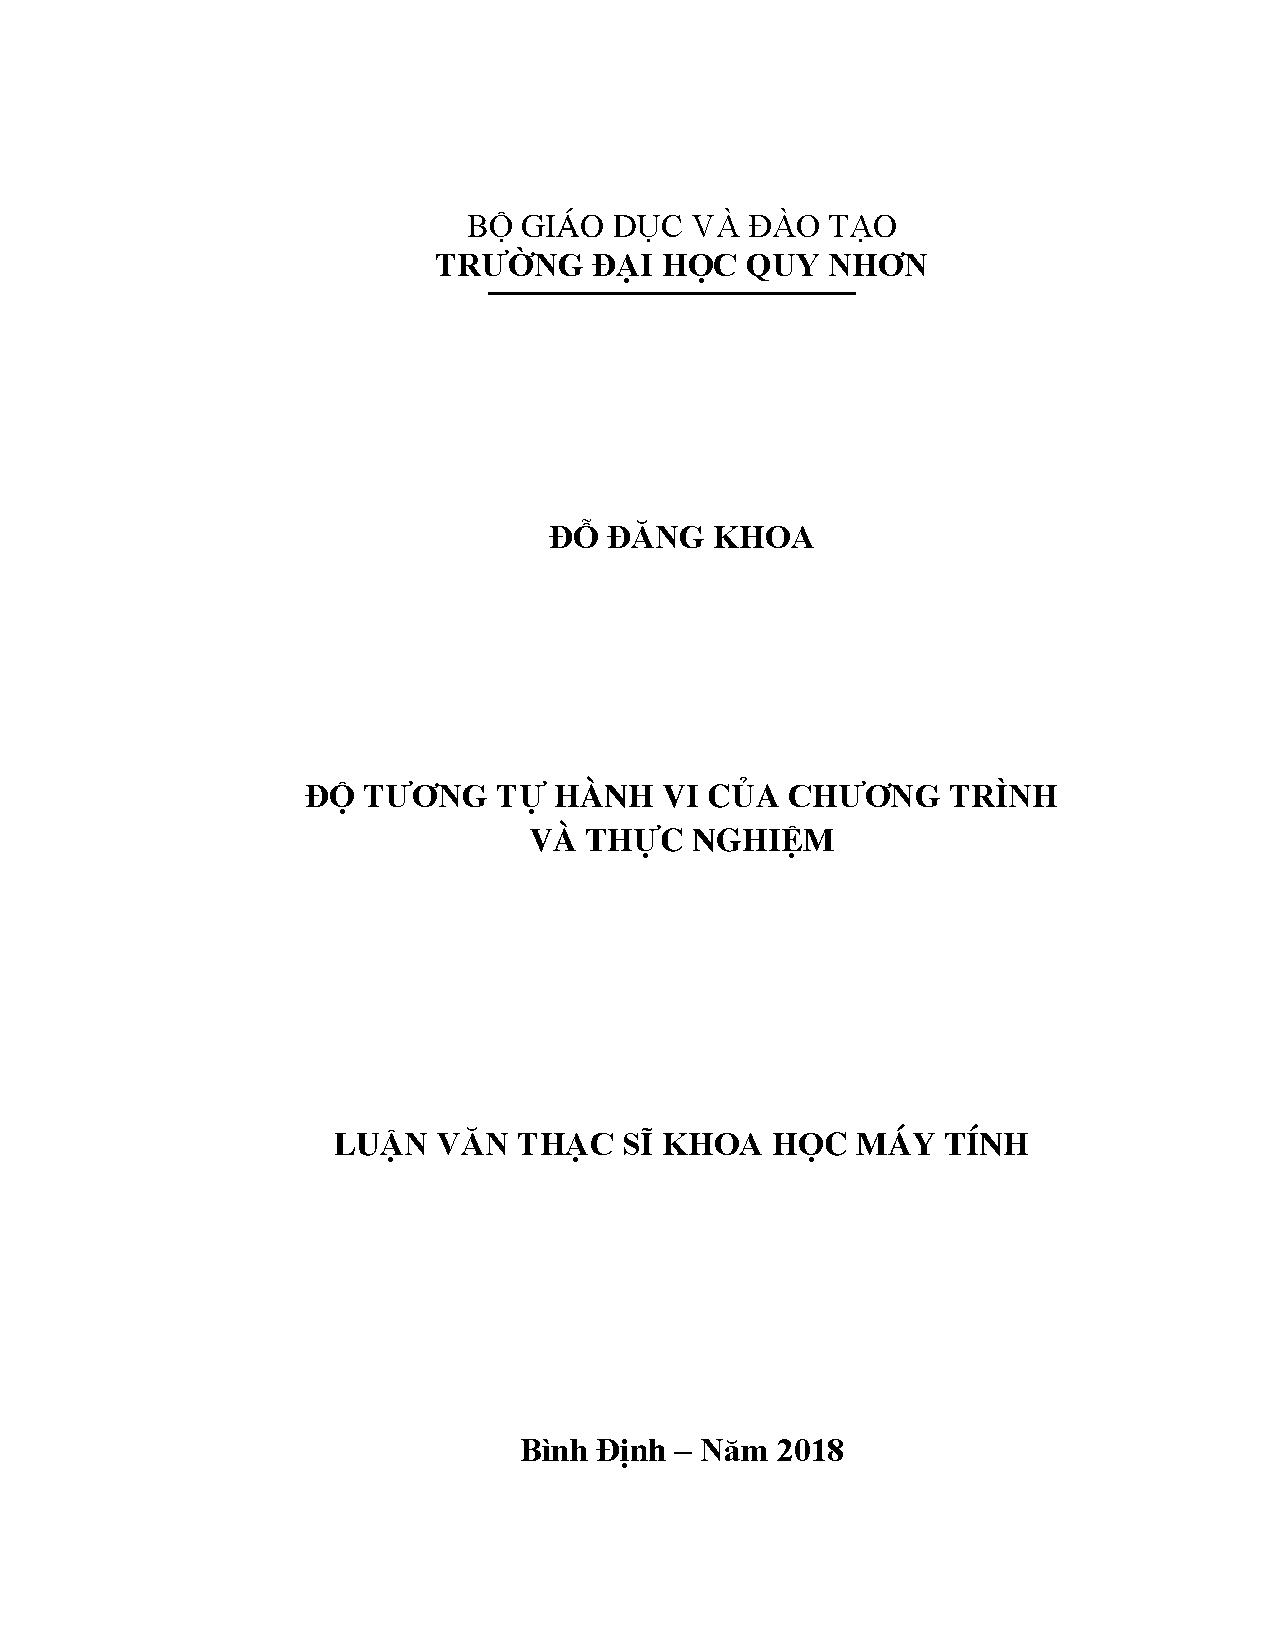
\includepdf[pages=-]{trangbia.pdf}
% \pagenumbering{gobble} % Trước trang không đánh số thứ tự 
% \pagenumbering{roman} % Trước trang đánh số la mã
% \setcounter{page}{1}
%\pagenumbering{arabic} % Trước trang đánh số thứ tự thêm 2 dòng này
%\setcounter{page}{1}   % Trước trang đánh số thứ tự thêm 2 dòng này - số trang bắt đầu bằng 3
\chapter*{LỜI CAM ĐOAN}
\input{Loicamdoan}
\chapter*{LỜI CẢM ƠN}

Tôi xin chân thành cảm ơn sự hướng dẫn, chỉ dạy và giúp đỡ tận tình của các thầy cô giảng dạy sau đại học - Trường đại học Quy Nhơn.

Đặc biệt, tôi cảm ơn thầy TS.Phạm Văn Việt, giảng viên bộ môn Công nghệ phần mềm, khoa Công nghệ thông tin, Trường Đại học Quy Nhơn đã tận tình hướng dẫn truyền đạt những kiến thức và kinh nghiệm quý báu đễ giúp tôi có đầy đủ kiến thức và nghị lực hoàn thành luận văn này.

Và tôi xin cảm ơn bạn bè, đồng nghiệp và những người thân trong gia đình đã tin yêu, động viên giúp tôi thêm nghị lực trong quá trình học tập và nghiên cứu.

Mặc dù đã cố gắng rất nhiều trong việc thực hiện luận văn, song với thời gian có hạn, nên luận văn không thể tránh khỏi những thiếu sót và chưa hoàn chỉnh. Tôi rất mong nhận được ý kiến đóng góp của quý Thầy Cô và các bạn.

Một lần nữa, tôi xin chân thành cảm ơn!.


\begin{tabu} to 1.0 \textwidth {  X[c] X[c]  X[c]  X[c]  }

	 & &  & \textbf{HỌC VIÊN} \\
	 \\ \\ \\ \\ \\ \\ \\ \\ \\ \\ \\ 
	 & &  & \textbf{Đỗ Đăng Khoa}  \\
         
       \end{tabu}



\newpage
\tableofcontents
%======================================================================
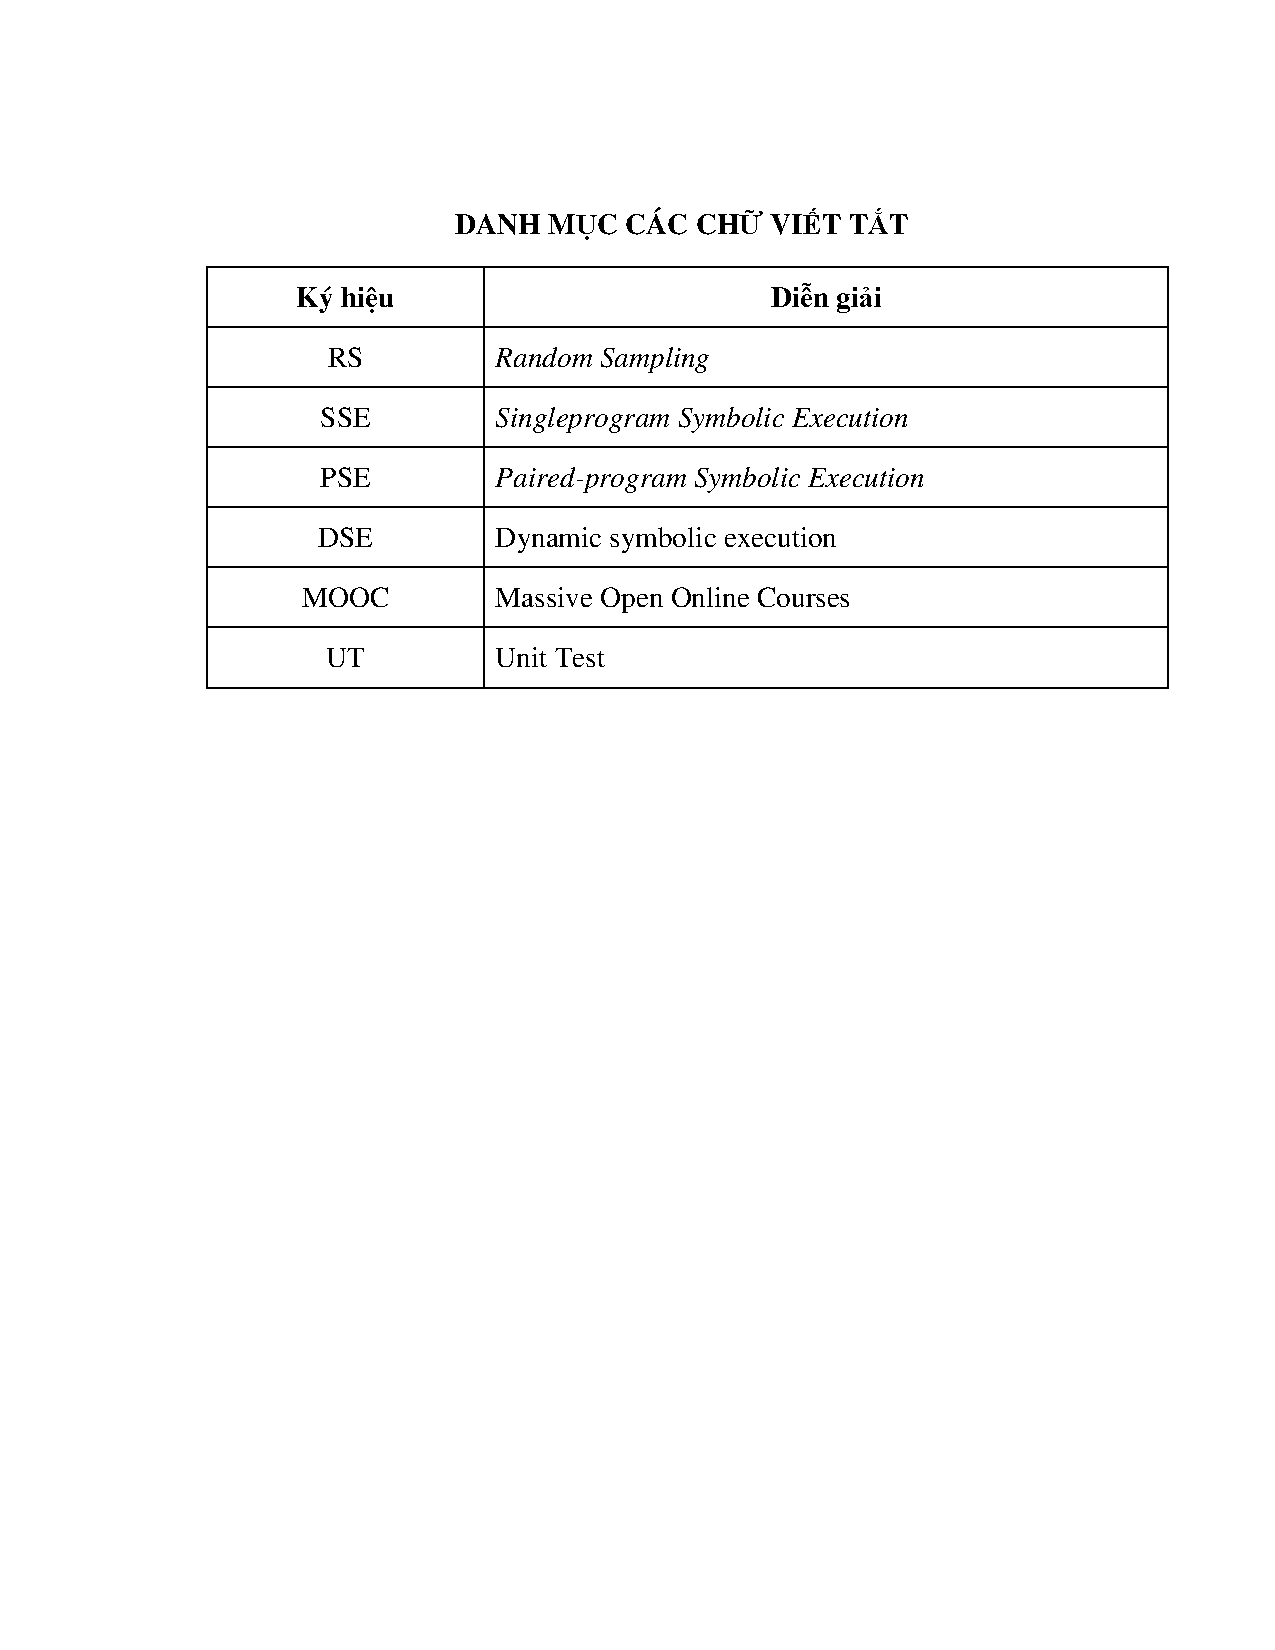
\includepdf[pages=1]{Danhmuckyhieu.pdf}
\newpage
\chapter{GIỚI THIỆU}
Chương này trình bày lý do chọn đề tài -- sự cần thiết đo độ tương tự
giữa các chương trình máy tính -- cùng mục tiêu nghiên cứu, đối tượng và phạm
vi nghiên cứu, cũng như những nghiên cứu có liên quan đến đề tài.

\section{Lý do chọn đề tài}

Hiện nay, ngành Công nghệ thông tin đang có xu hướng phát triển mạnh
mẽ và học trực tuyến ngày càng trở nên phổ biến. Một số chương trình
đào tạo trực tuyến nổi tiếng như
\href{https://www.coursera.org/course/saas}{Massive Open Online
  Courses (MOOC)} \cite{mooc}, \href{https://www.edx.org/}{edX}
\cite{edx}, \href{https://www.coursera.org/}{Coursera}
\cite{coursera}, \href{http://www.udacity.com/}{Udacity}
\cite{Udacity} (Hình \ref{fig:progarming-online}) ngày càng có nhiều người tham gia. Ngoài ra, một số
chương trình hỗ trợ rèn luyện kỹ năng lập trình trực tuyến như
\href{https://www.pexforfun.com/}{Pex4Fun} \cite{Pex4Fun} hay
\href{https://www.microsoft.com/en-us/research/project/code-hunt/}{Code
  Hunt} \cite{CodeHunt} cũng thu hút nhiều sự quan tâm của nhiều
người. 

\begin{figure}[h]
	\centering
	
\includegraphics[scale=.4]{topMOOC.png}
	\caption{Một số chương trình đào tạo trực tuyến nổi tiếng}
	\label{fig:progarming-online}		
\end{figure}

Một trong những thách thức của việc đào tạo lập trình trực tuyến là
tổ chức những lớp học có quy mô lớn, trong khi đó vẫn
đảm bảo chất lượng đào tạo. Thông thường, những khóa học trực tuyến
có nhiều học viên tham gia, hàng trăm thậm chí hàng ngàn, 
nhưng số người phụ trách giảng dạy không nhiều. Sự hạn chế về
số người phụ trách này có ảnh hưởng rất nhiều đến chất lượng đào
tạo. Về phía người giảng dạy, để xếp hạng học viên hay cung cấp những
phản hồi đối với từng lời giải của học viên đòi hỏi người dạy phải đọc hiểu
toàn bộ mã lệnh do học viên viết. Công việc này dường như quá nặng
nhọc nhưng không thể bỏ qua hoặc trì hoãn vì như vậy sẽ không thể nắm bắt
được tiến bộ của học viên. Ngoài ra, học viên đến từ rất
nhiều nơi trên thế giới nên thời gian học cũng khác nhau. Những lúc 
gặp khó khăn trong việc viết mã chương trình, người học có thể tìm kiếm sự
trợ giúp từ bạn bè hoặc những người có kinh nghiệm. Tuy
nhiên, không phải lúc nào cũng có người bên cạnh để giúp
đỡ cho họ, ảnh minh họa Hình \ref{fig:Retry}. 

\begin{figure}[h]
	\centering
	
\includegraphics[scale=.8]{Retry.png}
	\caption{Những khó khăn của người dạy và người học}
	\label{fig:Retry}		
\end{figure}

Thách thức trên có thể giải quyết nếu có được công cụ tự động hóa việc
so sánh giải pháp của học viên đưa ra so với giải pháp của giáo viên
xem chúng có tương đương không, hay tương tự nhau ở mức độ nào. Sự
tương đương giữa hai chương trình được hiểu theo nghĩa chúng cho ra
cùng kết quả nếu nhận vào cùng dữ liệu. Việc chuyển đổi từ dữ liệu vào
thành dữ liệu ra của một chương trình có thể xem là \emph{hành vi} của
nó. Công cụ này có thể giúp người dạy đánh giá xếp hạng giải pháp của
học viên dựa vào giải pháp của mình. Ngoài ra, công cụ còn có thể giúp
đánh giá được tiến bộ của người học, giúp đưa ra những gợi ý lập
trình cho học viên,\dots

Chúng tôi nhận thấy vấn đề cốt lõi để xây dựng công cụ này là làm sao
đo được độ tương tự về hành vi giữa hai chương trình. Đó là lý do tôi 
chọn đề tài \emph{``Độ tương tự hành vi của chương trình và thực nghiệm''}. 
Đề tài này sẽ làm rõ hành vi của chương trình, độ tương tự về hành vi của 
chương trình và một số phương pháp đo độ tương tự về hành vi.

\section{Đối tượng, phạm vi, phương pháp nghiên cứu}
\subsection{Mục tiêu nghiên cứu}

Mục tiêu nghiên cứu chính của luận văn là tìm cách đánh giá độ tương tự về 
hành vi giữa hai chương trình máy tính và được cụ thể hóa thành những mục tiêu sau:
\begin{itemize}
\item Tìm hiểu sự tương tự hành vi của chương trình;
\item Tìm hiểu kỹ thuật, công cụ sinh test case tự động và áp dụng để
  đo độ tương tự về hành vi;
\item Tìm cách kết hợp các kỹ thuật đo với nhau;
\item Đánh giá kết quả thực nghiệm.
\end{itemize}

\subsection{Đối tượng, phạm vi nghiên cứu}

\subsubsection*{Đối tượng nghiên cứu}

Đối tượng nghiên cứu chính trong luận văn này gồm:
\begin{itemize}
\item Kỹ thuật sinh Test Case
\item Các kỹ thuật đo độ tương tự hành vi
\item Ứng dụng của các kỹ thuật đo độ tương tự hành vi
\end{itemize}
	
\subsubsection*{Phạm vi nghiên cứu}
\begin{itemize}
\item Đo độ tương tự hành vi dựa vào Test Case
\item Thực nghiệm, đánh giá trên các chương trình C\#
\end{itemize}


\subsection{Phương pháp nghiên cứu, thực nghiệm}
\subsubsection*{Nghiên cứu lý thuyết}
\begin{itemize}
\item Độ tương tự hành vi
\item Một số kỹ thuật sinh Test Case tự động
\item Kỹ thuật đo độ tương tự hành vi dựa trên Test Case
\item So sánh, kết hợp các phép đo độ tương tự hành vi
\end{itemize}
		
\subsubsection*{Thực nghiệm}
\begin{itemize}
\item Tiến hành cài đặt các kỹ thuật đo độ tương tự hành vi
\item Thực nghiệm trên dữ liệu thực của CodeHunt, và một số dữ liệu thử khác
\item Phân tích, đánh giá dựa trên kết quả thực nghiệm
\end{itemize}


\section{Những nghiên cứu có liên quan}

Đề tài này liên quan đến những nghiên cứu về xếp hạng tự động, sự
tương đương giữa hai chương trình, phát hiện đạo code.

\subsection*{Xếp hạng tự động}
	
Trong bài báo \cite{alur2013automated} nhóm tác giả đề xuất một phương
pháp tự động so một automat hữu hạn đơn định chưa đúng của sinh viên
với automat hữu hạn đơn định của giáo viên dùng làm automat tham
chiếu. Cách tiếp cận này của các tác giả sử dụng các kỹ thuật đo sự
khác nhau về cả cú pháp và ngữ nghĩa giữa hai automat. Sự khác biệt về
cú pháp được đo qua khoảng cách chỉnh sửa (\emph{syntactic edit
  distance}) và sự khác biệt về ngữ nghĩa được đo dựa trên các
câu vào được đoán nhận bởi automat (\emph{accepted string
  inputs}). Mặc dù cách tiếp cận của nhóm tác giả bài báo và tác giả
luận văn đều sử dụng khái niệm về độ tương tự về ngữ nghĩa, cách tiếp
cận của bài báo dùng cho automat hữu hạn đơn định trong khi các độ đo
trong luận văn dùng cho các chương trình máy tính.

Một bài báo khác liên quan đến chủ đề này là \cite{singh2013automated}. 
Trong đó, nhóm tác giả đề xuất phương pháp tự động
xác định số sửa lỗi tối thiểu cần thực hiện trên chương trình của sinh 
viên (chưa đúng) sao cho khớp với giải pháp tham chiếu của giáo viên. 
Cách tiếp cận này cung cấp cách sử lỗi thông qua việc tính khoảng cách 
cú pháp tối thiểu (\emph{minimal syntactic distance}) giữa chương trình 
sai với chương trình tham chiếu, trong khi đó luận văn tập trung vào đo 
độ tương tự về ngữ nghĩa của hai chương trình dựa vào các hành vi vào/ra. 
Các độ đo trong luận văn có thể nhận biết độ tương tự giữa các chương trình 
có cấu trúc cú pháp khác nhau.

Ngoài ra, trước những nghiên cứu vừa nêu được đưa ra, trong bài báo
\cite{wang2007semantic}, tác giả đề xuất một giải pháp đo độ tương tự
về ngữ nghĩa của hai chương trình thông qua việc chuyển đổi chương
trình của học viên và chương trình tham chiếu của giáo viên về một
dạng chung nhưng không thay đổi ngữ nghĩa, đó là đồ thị phụ thuộc
(\emph{dependence graphs}), rồi tiến hành so sánh hai đồ thị để tính
toán sự tương đồng. Thay vì so sánh các đồ thị, cách tiếp cận của đề
tài này là so sánh các cặp đầu vào, đầu ra của các chương trình để
tính toán các điểm tương đồng về hành vi.
	
\subsection*{Kiểm tra sự tương đương giữa hai chương trình}

Có một số phương pháp kiểm tra sự tương đương về ngữ nghĩa/hành vi của
các chương trình bằng cách sử dụng đồ thị phụ thuộc
\cite{bates1993incremental,binkley1992using}, sự phụ thuộc giữa giá
trị đầu vào và đầu ra \cite{jackson1994semantic}. Tất cả các cách tiếp
cận để kiểm tra độ tương đương này đều trả về giá trị logic
đúng/sai. Tuy nhiên, ngoài việc kiểm tra sự tương đương, giải pháp
trong luận văn này còn có thể đo được độ tương tự giữa hai chương
trình.

Phương pháp tự động xác định những đoạn mã tương đương nhau về chức
năng thông qua các phép thử ngẫu nhiên
\cite{jiang2009automatic}. Cách tiếp cận này xem xét hai đoạn mã có
tương đương nhau hay không thông qua giá trị đầu vào và đầu ra, không
quan tâm đến cấu trúc và cú pháp của chúng. Độ đo RS trong luận văn này 
cũng tương tự với cách tiếp cận trong bài báo. Tuy nhiên, luận văn này 
các đưa ra hai phương pháp đo khác, dựa trên kỹ thuật thực thi biểu 
trưng chương trình DSE (\emph{Dynamic Symbolic Execution}).
		
\subsection*{Phát hiện đạo code}

Những nhà nghiên cứu đã đề xuất cách tiếp cận cho việc tính toán
độ tương tự giữa các biến thể của các đoạn mã lệnh để tự động nhận
diện đạo code, như sử dụng cây cú pháp trừu tượng
\cite{baxter1998clone}, đồ thị phụ thuộc của chương trình
\cite{komondoor2001using}, các độ đo dựa trên các đơn vị cú pháp (như
các lớp, hàm) \cite{dang2012xiao} \cite{merlo2004linear}. Các tiếp cận
này tính toán độ tương tự bằng cách phân tích tĩnh các đoạn mã lệnh
còn cách tiếp cận trong luận văn về việc tính độ tương tự bằng cách
thực thi chương trình để sinh ra các cặp dữ liệu vào/ra, làm cơ sở để
tính toán.
	
\section*{Tổng kết chương}

Ngày nay, những chương trình đào tạo trực tuyến ngày càng có nhiều
người tham gia, có thể lên đến hàng trăm, thậm chí hàng ngàn người mỗi
lớp. Thách thức quan trọng là làm sao tổ chức được các lớp có quy mô
lớn nhưng vẫn đảm bảo chất lượng giáo dục trong điều kiện số lượng
người tham gia giảng dạy cho mỗi lớp có hạn chế. Phương pháp đo độ
tương tự về hành vi giữa hai chương trình máy tính làm cơ sở để xây
dựng công cụ tự động hóa nhằm giảm thiểu công sức người dạy trong việc
đánh giá xếp hạng kết quả học tập của học viên cũng như đưa ra những
gợi ý hỗ trợ cho người học trong quá trình viết chương trình.
Chương \ref{chap:intro} cho thấy sự cần thiết của đề tài cũng như đối 
tượng, phạm vi và phương pháp nghiên cứu. Ngoài ra, chương này còn trình 
bày một số nghiên cứu có liên quan về việc xếp hạng tự động, kiểm tra sự 
tương đương, phát hiện đạo code.

Phần còn lại của luận văn được tổ chức thành ba chương. Chương \ref{chap:behaviors}
tập trung làm rõ về hành vi của chương trình, Chương \ref{chap:method} những phương
pháp đo độ tương tự về hành vi, Chương \ref{chap:results} trình bày
kết quả thực nghiệm cùng một số vấn đề liên quan.





%%% Local Variables:
%%% mode: latex
%%% TeX-master: "Main"
%%% End:


\chapter{TƯƠNG TỰ VỀ HÀNH VI GIỮA CÁC CHƯƠNG TRÌNH}
Chương này tập trung làm rõ hành vi của chương trình, độ tương tự về
hành vi giữa hai chương trình và các phương pháp đo độ tương tự về
hành vi, sẽ được trình bày trong Phần \ref{sec:behavior} và
\ref{sec:metrics}. Ngoài ra, chương này còn trình bày một số kiến thức
cơ sở về kiểm thử phần mềm và kỹ thuật sinh dữ liệu kiểm thử trong
Phần \ref{sec:base}.

\section{Kiến thức cơ sở}
\label{sec:base}

Ý tưởng chính của việc đo độ tương tự về hành vi giữa hai chương trình
máy tính là dựa trên tập dữ liệu vào, đếm số lượng dữ liệu ra tương
ứng giống nhau giữa hai chương trình và đo tỷ lệ tương tự. Dữ liệu vào
phải được chọn sao cho phủ nhiều nhất miền vào của chương trình. Về cơ
bản, độ tương tự này được đo dựa trên dữ liệu các ca kiểm thử. Chương
này trình bày ngắn gọn về kiểm thử phần mềm cùng việc sinh dữ liệu
kiểm thử, chủ yếu tập trung vào phương pháp thực thi biểu trưng một
chương trình (\emph{DSE -- Dynamic Symbolic Execution}) nhằm giúp tăng độ phủ
của dữ liệu thử.

\subsection{Kiểm thử phần mềm}
Hiện nay, ngành công nghiệp phần mềm giữ vai trò khá quan trọng. Một
số nước có nền công nghệ thông tin phát triển thì ngành công nghiệp
phần mềm có khả năng chi phối cả nền kinh tế. Vì vậy, việc đảm bảo
chất lượng phần mềm trở nên cần thiết hơn bao giờ hết.

Quá trình phát hiện và khắc phục lỗi của phần mềm là một công việc đòi hỏi nhiều nỗ lực, công sức, phát sinh thêm nhiều chi phí trong việc phát triển phần mềm. Một sản phẩm phần mềm đạt chất lượng cao, đáp ứng được yêu cầu của người sử dụng sẽ được nhiều người biết đến, nó mang lại hiệu quả tích cực trong công việc của người sử dụng. Ngược lại, một phần mềm kém chất lượng sẽ gây thiệt hại về kinh tế, ảnh hưởng đến công việc của người sử dụng. Vì vậy, yêu cầu đặt ra đó là một sản phẩm phần mềm phải đảm bảo được sự ổn định, không phát sinh lỗi trong quá trình sử dụng.

Kiểm thử phần mềm chính là một quá trình hoặc một loạt các quy trình
được thiết kế nhằm đảm bảo mã máy tính chỉ làm những gì nó được thiết
kế và không làm bất cứ điều gì ngoài ý muốn \cite{myers2011art}. Đây
là một bước quan trọng trong quá trình phát triển một phần mềm, giúp
cho nhà phát triển phần mềm và người sử dụng thấy được hệ thống đã đáp
ứng được yêu cầu đặt ra.

\subsubsection{Các phương pháp kiểm thử}

Có nhiều phương pháp để kiểm thử phần mềm, trong đó hai phương pháp
kiểm thử chính là \emph{kiểm thử tĩnh} và \emph{kiểm thử động}.

\emph{Kiểm thử tĩnh (Static testing)} là phương pháp kiểm thử phần mềm
bằng cách duyệt lại các yêu cầu, các đặc tả và mã lệnh chương trình
bằng tay, thông qua việc sử dụng giấy, bút để kiểm tra tính logic từng
chi tiết mà không cần chạy chương trình. Kiểu kiểm thử này thường được
sử dụng bởi chuyên viên thiết kế, người viết mã lệnh chương
trình. Kiểm thử tĩnh cũng có thể được tự động hóa bằng cách thực hiện
kiểm tra toàn bộ hệ thống thông qua một trình thông dịch hoặc trình
biên dịch, xác nhận tính hợp lệ về cú pháp của chương trình.
		
\emph{Kiểm thử động (Dynamic testing)} là phương pháp kiểm thử thông
qua việc thực thi chương trình để kiểm tra trạng thái tác động của
chương trình, dựa trên các ca kiểm thử xác định các đối tượng kiểm thử
của chương trình. Đồng thời, kiểm thử động sẽ tiến hành kiểm tra cách
thức hoạt động của mã lệnh, tức là kiểm tra phản ứng từ hệ thống với
các biến thay đổi theo thời gian. Trong kiểm thử động, phần mềm phải
được biên dịch và chạy, và bao gồm việc nhập các giá trị đầu vào và
kiểm tra giá trị đầu ra có như mong muốn không.

Trong luận văn này, độ tương tự về hành vi giữa hai chương trình được
đo thông qua việc thực thi hai chương trình, tức là sử dụng phương
pháp \emph{kiểm thử động}.
	
\subsubsection{Các chiến lược kiểm thử}

Hai chiến lược kiểm thử phần mềm được sử dụng nhiều nhất đó là \emph{kiểm thử hộp đen} và \emph{kiểm thử hộp trắng}.
	
\emph{Kiểm thử hộp đen (black box)} là một chiến lược kiểm thử với
cách thức hoạt động chủ yếu dựa vào hướng dữ liệu inputs/outputs của
chương trình, xem chương trình như là một ``hộp đen''. Chiến lược kiểm
thử này hoàn toàn không quan tâm về cách xử lý và cấu trúc bên trong
của chương trình, nó tập trung vào tìm các trường hợp mà chương trình
không thực hiện theo các đặc tả. Tuy nhiên, phương pháp kiểm thử này
cũng có mặt hạn chế của nó, kiểm thử viên không biết các phần mềm cần
kiểm tra thực sự được xây dựng như thế nào, cố gắng viết rất nhiều ca
kiểm thử để kiểm tra một chức năng của phần mềm nhưng lẽ ra chỉ cần
kiểm tra bằng một vài ca kiểm thử, hoặc một số phần của chương trình
có thể bị bỏ qua không được kiểm tra.

Do vậy, kiểm thử hộp đen có ưu điểm là đánh giá khách quan, mặt khác
nó lại có nhược điểm là thăm dò mù. Trong phần nghiên cứu của đề tài,
kiểm thử hộp đen cũng được sử dụng như một phương pháp đo độ tương tự
hành vi của các chương trình.
		
\emph{Kiểm thử hộp trắng (white box)} là một chiến lược kiểm ngược lại
với kiểm thử hộp đen, còn gọi là kiểm thử hướng logic của phần
mềm. Cách kiểm thử này cho phép tạo ra dữ liệu thử nghiệm từ việc kiểm
tra, khảo sát cấu trúc bên trong và kiểm thử tính logic của chương
trình. Dữ liệu thử nghiệm có độ phủ lớn, đảm bảo tất cả các đường dẫn,
hoặc các nhánh của chương trình được thực hiện ít nhất một lần, khắc
phục được những nhược điểm thăm dò mù trong cách kiểm thử hộp đen.

\subsection{Kỹ thuật Dynamic symbolic execution}
\label{sec:dse}

Dynamic symbolic execution (DSE) là một kỹ thuật sinh dữ liệu thử bằng
cách duyệt tự động tất cả các đường đi có thể của chương trình bằng
cách chạy chương trình với nhiều giá trị đầu vào khác nhau để tăng độ
phủ của dữ liệu thử được sinh ra \cite{xie2009fitness}.

Dựa trên kiểu dữ liệu của các tham số đầu vào của chương trình, kỹ
thuật DSE sẽ tạo ra các giá trị đầu vào cụ thể và thực thi chương
trình với các giá trị cụ thể vừa tạo. Trong quá trình thực thi, DSE sẽ
ghi nhận lại ràng buộc tại các nút rẽ nhánh của chương trình, phủ định
lại các ràng buộc này và sinh các giá trị đầu vào thỏa các điều kiện
ràng buộc vừa được ghi nhận. Với một giá trị đầu vào cụ thể, DSE sẽ
thực thi chương trình và duyệt được một đường đi cụ thể, quá trình
thực thi này sẽ lặp lại cho đến khi duyệt hết tất cả các đường đi của
chương trình. Thuật toán Algorithm~\ref{alg:DSE} mô tả cách thức hoạt
động tạo tập dữ liệu đầu vào thử nghiệm của kỹ thuật DSE.

\begin{algorithm}
	\caption{Thuật toán Dynamic symbolic execution}
	\label{alg:DSE}
	\begin{algorithmic}
        \item Set J:= $\varnothing $ \Comment{J: Tập hợp các đầu vào
            của chương trình phân tích}
        \item loop \subitem Chọn đầu vào i $\notin $ J \Comment{Dừng
            lại nếu không có i nào được tìm thấy} \subitem Xuất ra i
          \subitem Thực thi P(i); lưu lại điều kiện đường đi C(i); suy
          ra C'(i) \subitem Đặt J := J $\cup $ i
        \item end loop
	\end{algorithmic}
\end{algorithm}

Để hiểu rõ cách thức hoạt động tạo tập dữ liệu đầu vào thử nghiệm của kỹ thuật DSE chúng ta phân tích ví dụ trong Mã lệnh~\ref{lst:DSE} \cite{DSE}, với hàm \texttt{test\_me} có hai tham số đầu vào là \texttt{int x} và \texttt{int y} và hàm này không có giá trị trả về.

\lstinputlisting[caption={Ví dụ minh họa cách thức hoạt động của kỹ thuật DSE},label={lst:DSE}]{DSE.cs}	

Đầu tiên, DSE tạo hai tham số đầu vào thử nghiệm \texttt{(int x, int y)} có giá trị ngẫu nhiên, giả sử $x = 22$ và $y = 7$. Bên cạnh đó, DSE theo dõi tham số đầu vào của chương trình bằng một giá trị biểu trưng, với \texttt{x} bằng một số $x_{0}$ và \texttt{y} bằng một số $y_{0}$ (Hình \ref{fig:dse11}).

\begin{figure}[H]
	\caption{DSE tạo ngẫu nhiên các tham số đầu vào của chương trình}
	\label{fig:dse11}
	\begin{center}
		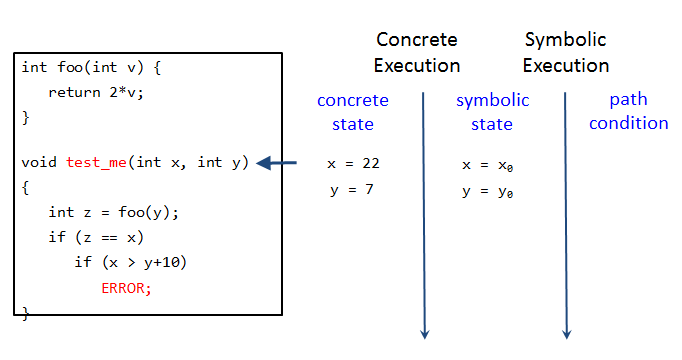
\includegraphics[scale=.7]{dse11.png}
	\end{center}	
\end{figure}

Tiếp theo, DSE thực thi dòng lệnh \texttt{(int z = foo(y))} nghĩa là gán  biến \texttt{z} bằng hàm \texttt{foo(y)}, lúc này biến $ z = 14 $ và trạng thái biểu trưng của biến \texttt{z} là $ z = 2*y_{0} $ (Hình \ref{fig:dse12})

\begin{figure}[H]
	\caption{DSE gán số nguyên \texttt{Z} bằng hàm \texttt{foo(y)}}
	\label{fig:dse12}
	\begin{center}
		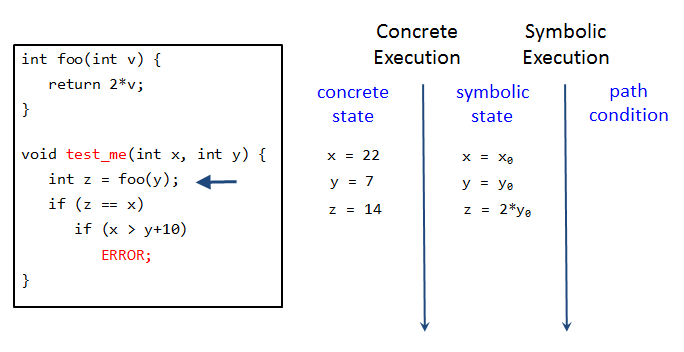
\includegraphics[scale=.7]{dse12.png}
	\end{center}	
\end{figure}

Tại câu lệnh \texttt{if(z == x)}, chúng ta thấy giá trị của \texttt{z} và \texttt{x} không bằng nhau, kết quả trả về của câu lệnh này sẽ là \texttt{fasle} dẫn đến kết thúc chương trình. Vì vậy, DSE sẽ lưu lại điều kiện ràng buộc \texttt{(z != x)} của đường dẫn này là $ 2*y_{0} != x_{0} $ (\ref{fig:dse13}).

\begin{figure}[H]
	\caption{DSE lưu lại điều kiện ràng buộc \texttt{(z != x)} của chương trình  }
	\label{fig:dse13}
	\begin{center}
		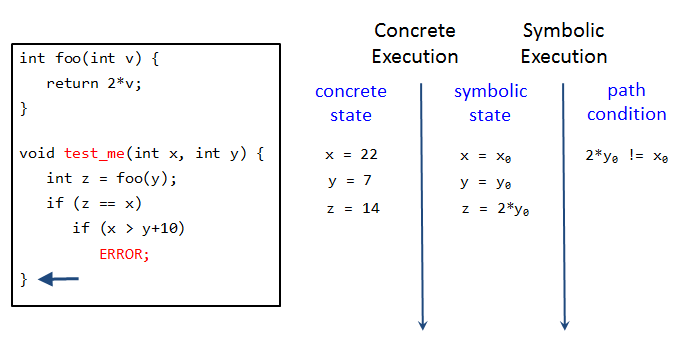
\includegraphics[scale=.7]{dse13.png}
	\end{center}	
\end{figure}

Sau khi kết thúc chương trình, DSE quay trở lại điểm vừa lưu điều kiện ràng buộc \texttt{(if(z == x))} để thực hiện phủ định điều kiện $2*y_{0} != x_{0}$ thành $2*y_{0} == x_{0}$. Sau đó DSE thực hiện tính toán và giải ràng buộc $2*y_{0} == x_{0}$, kết quả trả về là hai số nguyên có giá trị $ x_{0} = 2$, $ y_{0} = 1 $ thỏa ràng buộc (Hình \ref{fig:dse2}).

\begin{figure}[H]
	\caption{DSE tính toán và giải ràng buộc $2*y_{0} == x_{0}$}
	\label{fig:dse2}
	\begin{center}
		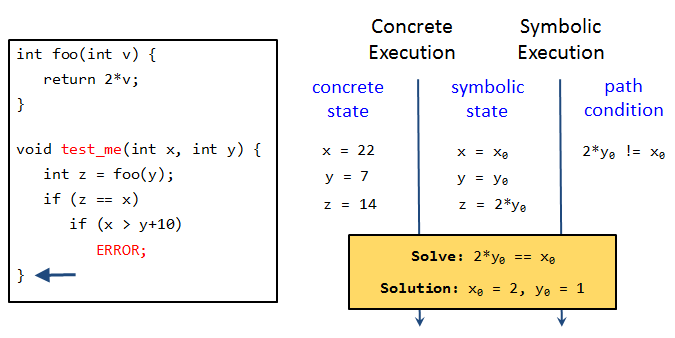
\includegraphics[scale=.7]{dse2.png}
	\end{center}	
\end{figure}

Sau đó, DSE khởi động lại hàm \texttt{test\_me} với các giá trị đầu vào cụ thể $x = 2$, $y = 1$ vừa tạo ra trước đó và tiếp tục theo dõi trạng thái biểu trưng các giá trị đầu vào với $x = x_{0}$ và $y = y_{0}$ (Hình \ref{fig:dse21}).

\begin{figure}[H]
	\caption{DSE khởi động lại hàm \texttt{test\_me}}
	\label{fig:dse21}
	\begin{center}
		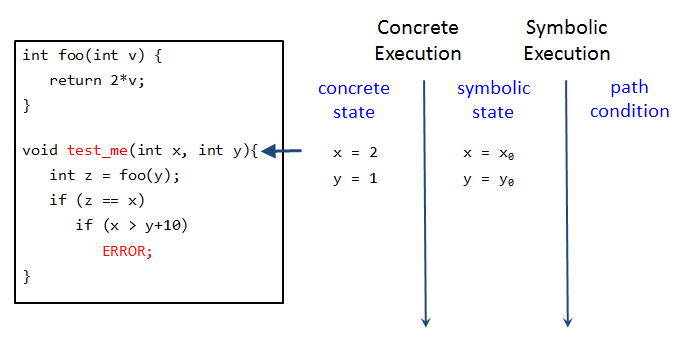
\includegraphics[scale=.7]{dse21.png}
	\end{center}		
\end{figure}


Tại câu lệnh gắn biến \texttt{z = foo(y)}, lúc này biến \texttt{z} sẽ có giá trị bằng $2$ và DSE thực hiện lưu trạng thái biểu trưng của biến \texttt{z} là $z = 2*y_{0}$ (Hình \ref{fig:dse22}).


\begin{figure}[H]
	\caption{DSE ghi nhận trạng thái biểu trưng của biến \texttt{z}}
	\label{fig:dse22}
	\begin{center}
		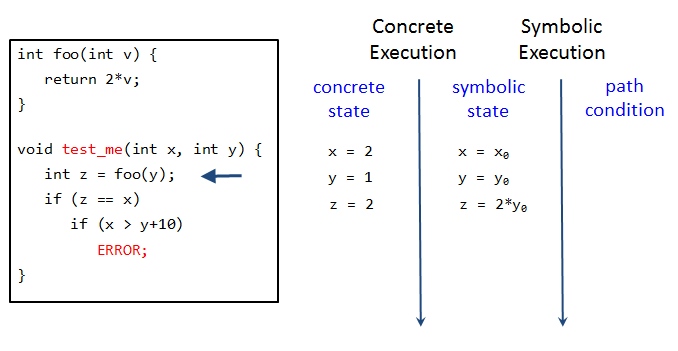
\includegraphics[scale=.7]{dse22.png}
	\end{center}		
\end{figure}

Tại nút rẽ nhánh \texttt{if(z == x)}, chúng ta thấy giá trị của biến $ z == x $ thỏa điều kiện nên chương trình tiếp tục thực thi theo nhánh điều kiện \texttt{true} và DSE ghi nhận ràng buộc $2*y_{0} == x_{0}$ cho nút nhánh này (Hình \ref{fig:dse23}).

\begin{figure}[H]
	\caption{DSE ghi nhận điều kiện ràng buộc $2*y_{0} == x_{0}$}
	\label{fig:dse23}
	\begin{center}
		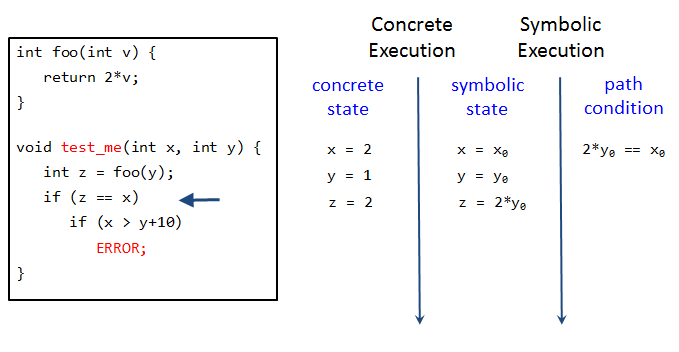
\includegraphics[scale=.7]{dse23.png}
	\end{center}	
\end{figure}

Tại nút rẽ nhánh tiếp theo \texttt{if(x > y+10)}, giá trị biến \texttt{x} bằng $2$, và $(y + 10)$ bằng $11$ nên chương trình sẽ thực thi theo nhánh \texttt{false} để kết thúc chương trình. Tại đây, DSE ghi nhận lại ràng buộc $x_{0} <= y_{0} + 10$ cho nút rẽ nhánh \texttt{if(x > y+10)} (Hình \ref{fig:dse24}).

\begin{figure}[H]
	\caption{DSE ghi nhận ràng buộc $x_{0} <= y_{0} + 10$}
	\label{fig:dse24}
	\begin{center}
		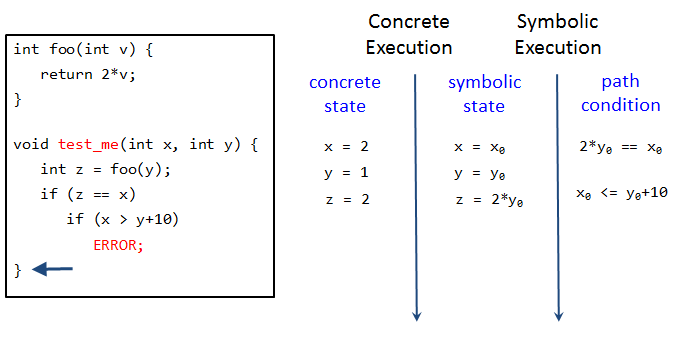
\includegraphics[scale=.7]{dse24.png}
	\end{center}		
\end{figure}

Vì đã đến cuối chương trình nên DSE quay lại nút nhánh gần nhất \texttt{if(x > y+10)} và thực hiện phủ định lại ràng buộc $x_{0} <= y_{0} + 10$ thành $ x_{0} > y_{0} + 10 $. Sau đó, DSE thực hiện giải ràng buộc $(2*y_{0} == x_{0}) and (x_{0} > y_{0} + 10)$ và tạo ra một giá trị đầu vào thỏa ràng buộc với $x_{0} = 30$ và $y_{0} = 15$ (Hình \ref{fig:dse3})

\begin{figure}[H]
	\caption{DSE thực hiện giải ràng buộc $(2*y_{0} == x_{0}) and (x_{0} > y_{0} + 10)$}
	\label{fig:dse3}
	\begin{center}
		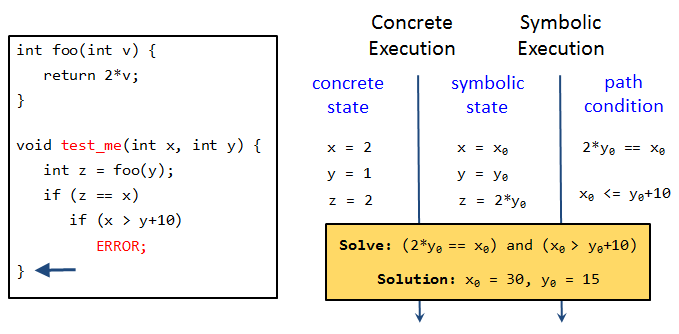
\includegraphics[scale=.7]{dse3.png}
	\end{center}
\end{figure}

Sau khi có giá trị đầu vào mới, DSE thực thi hàm \texttt{test\_me} một lần nữa với các giá trị đầu vào cụ thể $x = 30$ và $y = 15$ và tạo các trạng thái biểu trưng cho các biến đầu vào lần lượt $x = x_{0}$ và $y = y_{0}$ (Hình \ref{fig:dse31})

\begin{figure}[H]
	\caption{DSE thực thi hàm \texttt{test\_me} với $ x = 30 $ và $ y = 15 $}
	\label{fig:dse31}
	\begin{center}
		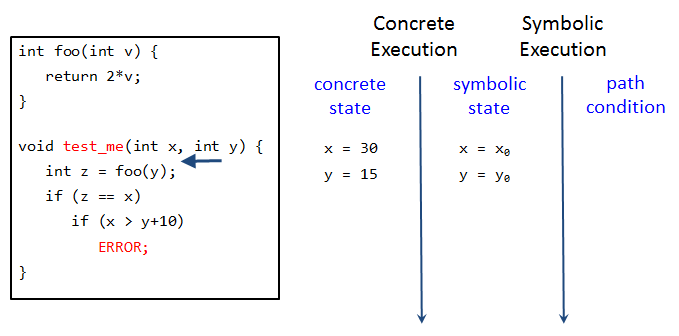
\includegraphics[scale=.7]{dse31.png}
	\end{center}
\end{figure}


Tại câu lệnh \texttt{z = foo(y)}, giá trị của biến \texttt{z} lúc này bằng $ 30 $ và trạng thái biểu trưng của biến \texttt{z} được khởi tạo $ z = 2*y_{0} $ như những lần trước đó (Hình \ref{fig:dse32})

\begin{figure}[H]
	\caption{DSE tạo trạng thái biểu trưng của biến \texttt{z}, với $ z = 30 $}
	\label{fig:dse32}
	\begin{center}
		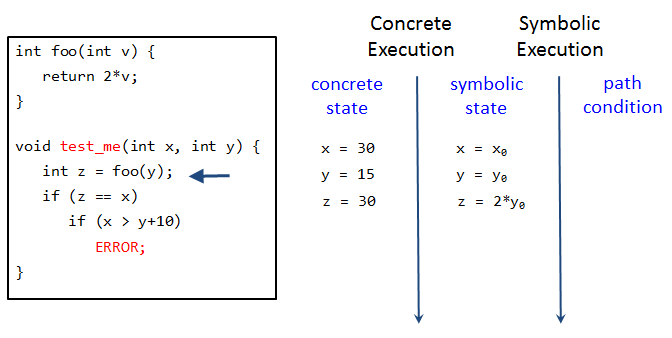
\includegraphics[scale=.7]{dse32.png}
	\end{center}
\end{figure}


Tại điểm nhánh \texttt{if(z == x)}, chúng ta thấy giá trị của biến \texttt{z} bằng giá trị của biến \texttt{x} nên chương trình thực thi theo nhánh \texttt{true} và DSE ghi nhận ràng buộc $ 2*y_{0} == x_{0} $ cho điểm nhánh này (Hình \ref{fig:dse33})

\begin{figure}[H]
	\caption{Ghi nhận điều kiện ràng buộc tại điểm nhánh \texttt{if(z == x)}}
	\label{fig:dse33}
	\begin{center}
		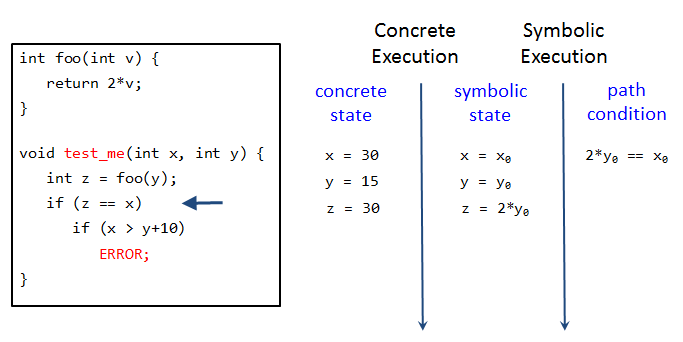
\includegraphics[scale=.7]{dse33.png}
	\end{center}
\end{figure}

Tại điểm nhánh tiếp theo \texttt{if(x > y+10)}, giá trị của biến $x = 30 $, biến $ y = 15 $ nên $(x >  y+10)$ thỏa điều kiện đường dẫn, chương trình sẽ thực thi theo nhánh \texttt{true} dẫn đến kết quả \texttt{ERROR}, lúc này DSE thực hiện ghi nhận lại ràng buộc $ x_{0} > y_{0}+ 10 $ cho nút rẻ nhánh \texttt{if(x > y+10)}. Vì chương trình thực thi đến \texttt{ERROR} và kết thúc chương trình nên chúng ta đã xác định được giá trị đầu vào cụ thể làm cho chương trình thực thi theo nhánh này với $x = 30$ và $y = 15$ (Hình \ref{fig:dse4}).

\begin{figure}[H]
	\caption{Đường dẫn của chương trình khi thực thi với giá trị $x = 30$ và $y = 15$}
	\label{fig:dse4}
	\begin{center}
		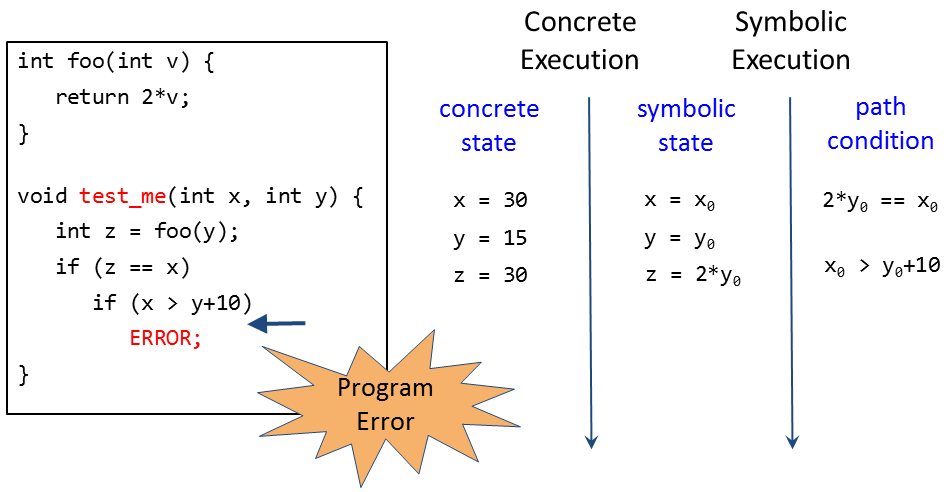
\includegraphics[scale=.6]{dse4.png}
	\end{center}	
\end{figure}

Sau 3 lần chạy chương trình, kỹ thuật DSE tạo ra tập các giá trị đầu vào $ [22,7] $, $ [2,1] $, $ [30,15] $ có độ phủ cao. Khi thực thi chương trình với tập giá trị đầu vào này tất cả các nhánh trong chương trình đều được thực thi. 
	
\subsection{Một số công cụ áp dụng DSE}	

Trên thế giới hiện có nhiều công cụ sử dụng kỹ thuật DSE để giải quyết
các ràng buộc và tạo ra các giá trị đầu vào có độ phủ cao như như Pex
\cite{tillmann2008pex} và SAGE \cite{godefroid2008automated}\dots và
những công cụ này được phát triển để có thể chạy được trên nhiều nền
tảng khác nhau. Chúng ta có thể tham khảo một số công cụ khác ở Bảng \ref{tbl:DSETools}.
		
\begin{table}[h]
  \centering
  \label{tbl:DSETools}
  \caption{Một số công cụ áp dụng kỹ thuật DSE}
  \begin{tabular} {|c|c|l|}
    \hline 
    \textbf{Tên Công cụ} & \textbf{Ngôn ngữ} & \textbf{Url} \\ 
    \hline 
    KLEE & LLVM & klee.github.io/ \\ 
    \hline 
    JPF	 & Java	& babelfish.arc.nasa.gov/trac/jpf \\
    \hline 
    jCUTE &	Java &	github.com/osl/jcute \\
    \hline 
    janala2	 & Java &	github.com/ksen007/janala2 \\
    \hline 
    JBSE	& Java	 & github.com/pietrobraione/jbse \\
    \hline 
    KeY &	Java &	www.key-project.org/ \\	
    \hline 
    Mayhem & 	Binary &	forallsecure.com/mayhem.html \\
    \hline 
    Otter &	C	& bitbucket.org/khooyp/otter/overview \\
    \hline 
    Rubyx & 	Ruby &	www.cs.umd.edu/~avik/papers/ssarorwa.pdf \\
    \hline 
    Pex	& .NET Framework	 & research.microsoft.com/en-us/projects/pex/ \\
    \hline 
    Jalangi2 &	JavaScript &	github.com/Samsung/jalangi2 \\
    \hline 
    Kite &	LLVM &	www.cs.ubc.ca/labs/isd/Projects/Kite/ \\
    \hline 
    pysymemu &	x86-64 / Native	 &github.com/feliam/pysymemu/ \\
    \hline 
    Triton	& x86 and x86-64 &	triton.quarkslab.com \\	
    \hline 
    BE-PUM &	x86	 & https://github.com/NMHai/BE-PUM	 \\	
    \hline
  \end{tabular} 
\end{table}
	
\section{Hành vi của chương trình }
\label{sec:behavior}

Trong luận văn này, hành vi của một chương trình là hành động biến đổi
một dữ liệu đầu vào thành đầu ra tương ứng. Chương trình được xem như
một hộp đen. Hành vi biến đổi của chương trình từ đầu vào sang đầu ra
là hành động một bước (\emph{one step action/big step}). Nghĩa là ta
không quan tâm đến sự thay đổi của dữ liệu qua từng bước nhỏ khi thực
hiện mỗi câu lệnh trong chương trình mà chỉ xem xét sự thay đổi qua
một bước lớn, xem tất cả các câu lệnh là một câu lệnh ghép.

Để hình thức hóa hành vi của một chương trình và sử dụng trong những
phần tiếp theo, ta tìm hiểu các định nghĩa hình thức liên quan đến
việc thực thi một chương trình, sự tương đương về hành vi giữa hai
chương trình, sự khác biệt về hành vi và độ tương tự về hành vi giữa
hai chương trình.
        
\subsection{Thực thi chương trình}

Việc thực thi một chương trình có thể xem là sự tương ứng mỗi giá trị vào với một giá trị ra, được nêu ra trong Định nghĩa \ref{def:progexe}.

\begin{definition}[Thực thi chương trình]
  \label{def:progexe}
  Cho $P$ là một chương trình, $I$ là tập hợp các trị đầu vào của $P$
  và $O$ là tập hợp các giá trị đầu ra của $P$. Thực thi chương trình
  P là ánh xạ:
  \[exec: P \times I \rightarrow O.
  \]
\end{definition}

Với giá trị đầu vào $i \in I$, sau khi thực thi chương trình $P$ trên
$i$ ta thu được giá trị đầu ra tương ứng $o \in O, o = exec(P, i)$.

\subsection{Tương đương về hành vi}

Hai chương trình được gọi là tương đương với nhau về hành vi nếu chúng
biến đổi cùng một giá trị vào thành cùng một giá trị ra đối với mọi
giá trị trên miền vào. Xét ví dụ hai chương trình trong Mã lệnh
\ref{lst:SwitchCase} và \ref{lst:IfElse}.

\begin{minipage}[t]{0.45\linewidth}
  \lstinputlisting[label={lst:SwitchCase}, caption =
  {Sử dụng \texttt{switch...case}}]{SwitchCase.cs}
\end{minipage}%
\hfill\vrule\hfill
\begin{minipage}[t]{0.45\linewidth}
  \lstinputlisting[label={lst:IfElse}, caption =
  {Sử dụng \texttt{if...else}}]{IfElse.cs}
\end{minipage}%

Mã lệnh \ref{lst:SwitchCase} và \ref{lst:IfElse} có cùng tham số đầu vào
\texttt{x} kiểu \texttt{int}, cùng tính toán và trả về giá trị
\texttt{y} phụ thuộc vào \texttt{x} theo cách: nếu \texttt{x = 1} thì
trả về \texttt{y + 4}, nếu \texttt{x = 2} thì trả về \texttt{2y}, còn
không thì trả về giá trị bình phương của \texttt{y}.

Rõ ràng hành vi của hai mã lệnh chương trình trên là tương đương vì
chúng trả về giá trị \texttt{y} giống nhau với cùng mỗi giá trị vào
kiểu số nguyên \texttt{x}, mặc dù chúng có cấu trúc khác nhau (Mã lệnh
\ref{lst:SwitchCase} sử dụng cấu trúc \texttt{switch...case}, Mã lệnh
\ref{lst:IfElse} sử dụng cấu trúc \texttt{if...else} để kiểm tra giá
trị đầu vào $x$). Sự tương đương về hành vi của hai chương trình được
hình thức hóa trong Định nghĩa \ref{def:equiv}.

\begin{definition}[Tương đương về hành vi]
  \label{def:equiv}
  Cho $P_{1}$ và $P_{2}$ là hai chương trình có cùng miền các giá trị
  đầu vào $I$. Hai chương trình này được gọi là tương đương khi và chỉ
  khi thực thi của chúng giống nhau trên mọi giá trị đầu vào trên $I$,
  ký hiệu là exec($P_{1}, I$) = exec($P_{2}, I$).
\end{definition}
	
\subsection{Khác biệt về hành vi}

Dựa vào Định nghĩa \ref{def:equiv} ta có thể suy ra hai chương trình
có hành vi khác nhau nếu chúng có miền giá trị đầu vào khác nhau, hoặc
có một vài giá trị vào làm cho thực thi của chúng khác nhau. Trong
phần này ta chỉ xét những chương trình có cùng miền giá trị vào. Ví dụ trong Hình \ref{fig:behavioral-diff} minh họa điều đó.

\begin{figure}[h]
  \centering
  \caption{Ví dụ sự khác biệt về hành vi}
  \label{fig:behavioral-diff}
  \begin{minipage}[t]{0.45\linewidth}
    \lstinputlisting[caption={Chương trình $ P_{1} $}, label={KBHV1}]{Khac_biet_HV_1.cs}
  \end{minipage}%
\hfill\vrule\hfill
\begin{minipage}[t]{0.45\linewidth}
  \lstinputlisting[caption={Chương trình $ P_{2} $}, label={KBHV2}]{Khac_biet_HV_2.cs}
\end{minipage}%
\end{figure}

Trong Hình \ref{fig:behavioral-diff}, hàm $F1$ và $F2$ có cùng miền
giá trị đầu vào kiểu \texttt{int}. Với mối giá trị vào \texttt{x}, giá
trị trả về của hàm $F1$ là $x - 10$ và của $F2$ là $x + 10$. Rõ ràng
hai hàm này có hành vi khác nhau. Mô tả hình thức về sự khác biệt hành
vi giữa hai chương trình được nêu ra trong Định nghĩa
\ref{def:equiv-diff}.

\begin{definition}[Sự khác biệt về hành vi]
  \label{def:equiv-diff}
  Cho $P_{1}$ và $P_{2}$ là hai chương trình có cùng miền các giá trị
  đầu vào $I$. Hai chương trình này được xem là có sự khác biêt về
  hành vi khi và chỉ khi thực thi của chúng khác nhau trên một vài giá
  trị đầu vào $i \in I$, ký hiệu là
  $exec(P_{1}, I) \neq exec(P_{2}, I)$.
\end{definition}

\subsection{Độ tương tự về hành vi}

Trong trường hợp hai chương trình không tương đương nhau về hành vi,
nghĩa là có sự khác biệt về hành vi giữa chúng, thì ta cần biết mức độ
tương tự giữa chúng là bao nhiêu. Thông tin này khá hữu ích, nó giúp
cho người dạy có thể đánh giá xếp hạng được giải pháp của người học
dựa vào giải pháp của mình đưa ra, hoặc có thể biết được mức độ hoàn
thiện của giải pháp do người học đưa ra. Xét độ tương tự về hành vi
của hai chương trình $P_{1}$ và $P_{2}$ được cho lần lượt trong Mã
lệnh \ref{TTHV1} và \ref{TTHV2}. Chúng ta dễ dàng thấy được hai hàm
$F1$ và $F2$ là không tương đương nhau trên toàn bộ miền giá trị vào
\texttt{int} mà chỉ tương đương trên miền các giá trị số nguyên
$E = [0,100] \cup \{-1\}$. Từ đó, ta có thể tính được độ tương tự về
hành vi của hai hàm này là $|E| / |\texttt{int}|$, trong đó
$|\mathtt{int}|$ là kích thước miền giá trị vào của hai hàm,
\texttt{int}.

\begin{figure}[H]
	\centering
	\caption{Ví dụ độ tương tự về hành vi}
	\label{fig:behavioral-sim}
	\begin{minipage}[t]{0.45\linewidth}
	  \lstinputlisting[label={TTHV1}, caption = {Chương trình  
	  	$P_{1}$}]{TuongTu_HV_1.cs}
	\end{minipage}%
	\hfill\vrule\hfill
	\begin{minipage}[t]{0.45\linewidth}
	  \lstinputlisting[label={TTHV2}, caption = {Chương trình  
	    $P_{2}$}]{TuongTu_HV_2.cs}
	\end{minipage}%
\end{figure}

Mô tả hình thức cho độ tương tự về hành vi giữa hai chương trình được
nêu ra trong Định nghĩa \ref{def:equiv-sim}. Trong định nghĩa này,
$I_s$ là tập lớn nhất các giá trị vào mà ở đó hai chương trình tương
đương về hành vi.
    
\begin{definition}[Độ tương tự về hành vi]
  \label{def:equiv-sim}
  Cho $P_{1}$ và $P_{2}$ là hai chương trình có cùng miền giá trị đầu
  vào $I$. Gọi $I_{s} \subseteq I$ là tập con của $I$ sao cho
  $exec(P_{1}, I_{s}) = exec(P_{2}, I_{s})$ và
  $\forall j \in I \setminus I_{s}, exec(P_{1}, j) \neq exec(P_{2},
  j)$. Khi đó, độ tương tự về hành vi giữa $P_1$ và $P_2$ là $|I_s|/|I|$.
\end{definition}

\section{Một số phép đo độ tương tự hành vi}
\label{sec:metrics}

Theo Định nghĩa \ref{def:equiv-sim}, để đo độ tương tự về hành vi của
hai chương trình ta cần xác định:
\begin{enumerate}
\item Số phần tử miền vào của hai chương trình
\item Số phần tử trên miền vào (cực đại) mà ở đó hai chương trình thực thi giống nhau.
\end{enumerate}
Dễ thấy, việc thứ $1$ tương đối đơn giản, chỉ cần cho thực thi hai
chương trình và so sánh kết quả. Khó khăn nằm ở công việc $2$. Với
những chương trình có miền vào nhỏ hoặc hữu hạn thì có thể thực hiện
việc này bằng cách vét cạn tất cả các khả năng. Tuy nhiên, với những
chương trình có miền vào cực lớn hoặc vô hạn thì việc vét cạn như vậy
hầu như bất khả thi. Để giải quyết vấn đề này, chúng ta cần đến kỹ
thuật sinh mẫu thử tự động sao cho đảm bảo bao phủ miền vào nhiều
nhất. Luận văn này áp dụng kỹ thuật thực thi biểu trưng đối với chương
trình (dynamic symbolic execution -- DSE) để giải quyết khó khăn này
(Xem Mục \ref{sec:dse}).

Phần còn lại của mục này trình bày ba phương pháp đo độ tương tự về
hành vi giữa hai chương trình: lấy mẫu ngầu nhiên, áp dụng DSE trên
đơn chương trình tham chiếu, áp dụng DSE trên chương trình hợp thành
từ chương trình giải pháp (\emph{do người học cung cấp}) và chương
trình tham chiếu (\emph{đưa ra bởi người dạy}).

\subsection{Lấy mẫu ngẫu nhiên}

Phương pháp đơn giản nhất để đo độ tương tự về hành vi giữa hai chương
trình là lấy ngẫu nhiên một số giá trị trên miền vào (\emph{Random
  Sampling -- RS}) và tính số lượng giá trị mà ở đó hai chương trình
thực thi giống nhau, từ đó tính mức độ tương tự. Chúng ta gọi phép đo
độ tương tự theo phương pháp này là \emph{Phép đo RS}, được mô tả hình thức
trong Định nghĩa \ref{def:RS-sim}.

\begin{definition}[Phép đo RS]
  \label{def:RS-sim}
  Cho $P_{1}$ và $P_{2}$ là hai chương trình có cùng miền giá trị đầu
  vào $I$, $I_{s}$ là tập con ngẫu nhiên của $I$, $I_{a}$ là tập con
  $I_{s}$ sao cho $exec(P_{1}, I_a) = exec(P_{2}, I_a)$ và
  $\forall j \in I_{s} \setminus I_{a}$, thì
  $exec(P_{1}, j) \neq exec(P_{2}, j)$. Độ tương tự về hành vi giữa
  hai chương trình theo phép đo RS được định nghĩa là
  $M_{RS}(P_{1}, P_{2}) = \left|I_{a}\right| \diagup
  \left|I_{s}\right| $.
\end{definition}

Từ Định nghĩa \ref{def:RS-sim}, chúng tôi xây dựng thuật toán để tính
độ tương tự theo phép đo RS như mô tả trong Algorithm \ref{alg:RS},
trong đó $I_s = Random(I)$ là thao tác chọn ngẫu nhiên một số giá trị
vào $I_s$ trong miền $I$. Trong phần thực nghiệm ở Chương
\ref{chap:results}, chúng tôi chọn số lượng giá trị ngẫu nhiên là
$200$, nghĩa là $|I_s| = 200$.

\begin{algorithm}[H]
  \caption{Phép đo RS}
  \label{alg:RS}
  \begin{algorithmic}
  \item $P_{1}, P_{2}:$ Là hai chương trình cần đo độ tương tự
  \item $I$: Miền giá trị đầu vào của $P_{1}, P_{2}$
  \item Set $I_{s} = Random(I)$ \Comment{$I_{s}$: Tập con ngẫu nhiên
      của $I$}
  \item Set $I_{a} = \emptyset$

    \For {$i \in I_s$}
        \If{ ($exec(P_{1}, i) = exec(P_{2}, i)$) } \State
        $I_{a} = I_{a} \cup i$
    \EndIf
    \EndFor
  \item
    $M_{RS}(P_{1}, P_{2}) = \left|I_{a}\right| \diagup
    \left|I_{s}\right| $.
  \end{algorithmic}
\end{algorithm}


Phép đo \textbf{RS} là một một phép đo đơn giản để tính độ tương tự về hành vi giữa hai chương trình. Vì không phải phân tích từng câu lệnh của chương trình mà chỉ quan tâm đến kiểu của miền giá trị vào để chọn một số giá trị ngẫu nhiên nên tốc độ xử lý tương đối nhanh và ít tốn tài nguyên hệ thống. Tuy nhiên, nhược điểm của phương pháp này là độ bao phủ của dữ liệu sinh ngẫu nhiên không cao. Chúng ta phân tích Mã lệnh \ref{RS1} và \ref{RS2} để thấy được hạn chế của phép đo \textbf{RS}.

\begin{figure}[h]
	\centering
	\caption{Ví dụ hạn chế của phép đo \texttt{RS}}
	\label{fig:Hanche-RS}
	\begin{minipage}[t]{0.45\linewidth}
		\lstinputlisting[label={RS1},caption = {Chương trình
			$P_{1}$}]{RS1.cs}
	\end{minipage}%
	\hfill\vrule\hfill
	\begin{minipage}[t]{0.45\linewidth}
		\lstinputlisting[label={RS2}, caption = {Chương trình
			$P_{2}$}]{RS2.cs}
	\end{minipage}% 
\end{figure}

Hai chương trình $P_{1}$ và $P_{2}$ có cùng tham số vào \texttt{x} kiểu \texttt{string}, cấu trúc mã lệnh hai chương trình gần giống nhau. Chương trình $P_{1}$ khác với chương trình $P_{2}$ khi có một điểm rẻ nhánh \texttt{if (x == "XYZ") return 0;}. Với điểm rẻ nhánh này, khả năng phép đo \textbf{RS} lấy ngẫu nhiên giá trị vào \texttt{x} có giá trị bằng \texttt{XYZ} trong miền vào kiểu \texttt{string} là rất thấp. Do đó chương trình $P_{1}$ có thể sẽ không thực thi nhánh \texttt{if (x == "XYZ") return 0}. Dữ liệu vào được lấy ngẫu nhiên trong phép đo RS trên miền vào của hai chương trình có thể sẽ không bao phủ hết các nhánh của chương trình.

\subsection{DSE trên chương trình tham chiếu}

Nhược điểm của phép đo RS được khắc phục bằng cách áp dụng kỹ thuật
DSE để tăng độ bao phủ của tập dữ liệu thử. Phép đo áp dụng DSE trên
chương trình tham chiếu, sau đây gọi tắt là SSE (\emph{Single program
  Symbolic Execution}), chỉ cần dựa vào chương trình tham chiếu để xác
định tập dữ liệu thử. Sự khác nhau giữa SSE và RS là SSE cần phần tích
các câu lệnh của chương trình trong khi đó RS chỉ quan tâm đến kiểu dữ
liệu vào. Mô tả hình thức cho phép đo SSE được nêu ra trong Định nghĩa
\ref{def:sse}.

\begin{definition}[Phép đo SSE]
  \label{def:sse}
  Cho $P_{1}$ và $P_{2}$ là hai chương trình có cùng miền giá trị đầu
  vào $I$, trong đó $P_{1}$ là chương trình tham chiếu. Gọi $I_{s}$ là
  tập các giá trị đầu vào được tạo bởi DSE trên $P_{1}$, và
  $I_{a} \subseteq I_s$ là tập con lớn nhất của $I_{s}$ sao cho
  $exec(P_{1}, I_a) = exec(P_{2}, I_a)$ và
  $\forall j \in I_{s} \setminus I_{a}, exec(P_{1}, j) \neq
  exec(P_{2}, j)$. Độ tương tự về hành vi giữa hai chương trình dùng
  phép đo SSE được định nghĩa là
  $M_{SSE}(P_{1}, P_{2}) = \left|I_{a}\right| \diagup
  \left|I_{s}\right| $.
\end{definition}

Thuật toán để đo độ tương tự dùng phép đo SSE được mô tả trong
Algorithm \ref{alg:sse}, trong đó $P_1$ là chương trình tham chiếu và
$DSE(P_{1})$ là hành động sinh dữ liệu thử cho chương trình $P_1$ áp
dụng kỹ thuật DSE.

\begin{algorithm}[h]
  \caption{Phép đo SSE}
  \label{alg:sse}
  \begin{algorithmic}
  \item $P_{1}, P_{2}:$ hai chương trình cần đo tương tự, $P_1$ là chương trình tham chiếu
  \item $I$: Miền giá trị đầu vào của $P_{1}, P_{2}$
  \item Set $I_{s} = DSE(P_{1})$ \Comment{$I_{s}$: Tập đầu vào của
      $P_{1}$ theo DSE}
  \item Set $I_{a} = \emptyset$
    \For{ ($i \in I_{s}$) }
    \If{ ($exec(P_{1}, i) = exec(P_{2}, i)$) } \State
    $I_{a} = I_{a} \cup i$
    \EndIf
    \EndFor
  \item
    $M_{SSE}(P_{1}, P_{2}) = \left|I_{a}\right| \diagup
    \left|I_{s}\right| $.
  \end{algorithmic}
\end{algorithm}

Để tính độ tương tự hành vi của hai chương trình với phép đo
\textbf{SSE}, chúng ta chọn chương trình mẫu làm chương trình tham
chiếu và áp dụng kỹ thuật \textbf{DSE} để tạo ra các đầu vào thử
nghiệm dựa trên chương trình tham chiếu. Sau đó thực thi cả hai chương
trình dựa trên các giá trị đầu vào thử nghiệm. Tỷ lệ số lượng các kết
quả đầu ra giống nhau của cả hai chương trình trên tổng số các giá trị
đầu vào thử nghiệm của chương trình tham chiếu là kết quả của phép đo
\textbf{SSE}.

Ngược lại với phép đo RS, phép đo SSE khám phá những đường đi khả thi
khác nhau trong chương trình tham chiếu để tạo dữ liệu đầu vào của
chương trình. Do đó, các đầu vào thử nghiệm này sẽ thực thi hết các
đường đi của chương trình tham chiếu và có khả năng phát hiện được
những chương trình cần tính có những hành vi khác so với chương trình
tham chiếu. Nhưng phép đo SSE vẫn còn hạn chế, đó là phép đo SSE không
xem xét đường đi của chương trình cần phân tích để tạo các giá trị đầu
vào thử nghiệm mà chỉ dựa vào các đầu vào thử nghiệm được phân tích từ
chương trình tham chiếu. Các đầu vào thử nghiệm này không bao phủ được
hết các hành vi của chương trình cần phân tích vì chương trình cần
phân tích có thể sẽ có những hành vi khác so với chương trình tham
chiếu. Một số chương trình có thể có những vòng lập vô hạn phụ thuộc
vào giá trị đầu vào nên SSE không thể liệt kê được tất cả các đường
đi của chương trình. Chúng ta xem xét và phân tích 2 đoạn Mã lệnh
\ref{SSE1} và \ref{SSE2} để thấy được hạn chế của phép đo SSE.
\begin{figure}[h]
	\centering
	\caption{Ví dụ hạn chế của phép đo SSE}
	\label{fig:hanche-SSE}
\begin{minipage}[t]{0.45\linewidth}
  \lstinputlisting[label={SSE1}, caption = {Chương trình
    $P_{1}$}]{SSE1.cs}
\end{minipage}%
\hfill\vrule\hfill
\begin{minipage}[t]{0.45\linewidth}
	\lstinputlisting[label={SSE2}, caption = {Chương trình $P_{2}$}]{SSE2.cs}
\end{minipage}%
\end{figure}

Hai đoạn Mã lệnh \ref{SSE1} và Mã lệnh \ref{SSE2} của hai chương trình
$P_{1}$ và $P_{2}$, chọn chương trình $P_{1}$ làm chương trình tham
chiếu, sử dụng kỹ thuật \textbf{DSE} để phân tích chương trình $P_{1}$
ta được tập các giá trị đầu vào thử nghiệm là ${(0, 1)}$. Trong khi
đó, phân tích chương trình $P_{2}$ chúng ta được tập các giá trị đầu
vào thử nghiệm của chương trình $P_{2}$ là ${(0, 1, 2)}$. Tập giá trị đầu vào thử nghiệm do phép đo \textbf{SSE} tạo ra thiếu giá trị đầu vào $2$ để có thể phủ hết các đường đi của chương trình $P_{2}$.

\subsection{DSE trên chương trình hợp thành}

Để giải quyết giới hạn của phép đo SSE khi tạo ra tập các giá trị đầu
vào thử nghiệm không thực thi hết các các đi của chương trình cần phân
tích, ta xây dựng một chương trình hợp thành kết hợp cả hai, được mô
tả trong Định nghĩa \ref{def:combination}.

\begin{definition}[Chương trình hợp thành]
  \label{def:combination}
  Cho $P_1$ và $_2$ là hai chương trình có cùng miền vào $I$, trong đó
  $P_1$ là chương trình tham chiếu. Hợp thành của hai chương trình là
  một chương trình mới $P_c = P_1 \oplus P_2$ có dạng
  $assert(exec(P_{1}, I) = exec(P_{2}, I))$, trong đó $assert(\dots)$
  là hàm đánh giá nhận vào một biểu thức điều kiện và đánh giá xem
  biểu thức đó đúng hay sai. Ký hiệu $exec(P_c,i) = \top$ để chỉ
  chương trình hợp thành $P_c$ thỏa hàm đánh giá, cũng có nghĩa là hai
  chương trình thành phần thực thi giống nhau trên đầu vào $i$.
\end{definition}

Phép đo độ tương tự về hành vi giữa hai chương trình áp dụng kỹ thuật
DSE trên chương trình hợp thành, từ đây gọi là phép đo PSE
(\emph{Paired program Symbolic Execution}), giải quyết giới hạn của
phép đo SSE bằng cách tạo một chương trình hợp thành giữa chương trình
cần phân tích với chương trình tham chiếu. Dựa trên chương trình hợp
thành, ta sử dụng kỹ thuật DSE để tạo ra đầu vào thử nghiệm cho cả hai
chương trình. Các đầu vào thử nghiệm này bao gồm các đầu vào thử
nghiệm đúng và không đúng. Các đầu vào thử nghiệm đúng là những giá
trị khi thực thi trên cả hai chương trình sẽ cho kết quả đầu ra như
nhau, ngược lại các đầu vào thử nghiệm không đúng là những giá trị khi
thực thi trên cả hai chương trình sẽ cho kết quả khác nhau. Do đó,
phép đo PSE được tính bằng tỷ lệ các giá trị đầu vào thử
nghiệm đúng trên tổng số các giá trị đầu vào được thử nghiệm.

Thuật toán mô tả cách đo độ tương tự về hành vi giữa hai chương trình theo phép đo PSE được mô tả trong Algorithm \ref{alg:pse}.

 \begin{algorithm}[h]
   \caption{Phép đo PSE}
   \label{alg:pse}
   \begin{algorithmic}
   \item $P_{1}, P_{2}$: hai chương trình cần đo tương tự, $P_1$ là
     chương trình tham chiếu
   \item $I$: Miền giá trị đầu vào của $P_{1}, P_{2}$
   \item $P_{3} = P_1 \oplus P_2$
   \item Set $I_{s} = DSE(P_{3})$ \Comment{$I_{s}$: Tập đầu vào của
       $P_{3}$ theo DSE}
   \item Set $I_{a} = \emptyset$ 
   		\For{$i \in I_{s}$}
     	\If{($exec(P_{1}, i) = exec(P_{2}, i)$) } 
     	\State $I_{a} = I_{a} \cup i$ 
     	\EndIf 
     	\EndFor
   \item
     $M_{PSE}(P_{1}, P_{2}) = \left|I_{a}\right| \diagup
     \left|I_{s}\right| $.
   \end{algorithmic}
 \end{algorithm}

Phép đo \textbf{PSE} đã cải thiện được hạn chế của phép đo
 \textbf{SSE} khi dữ liệu thử nghiệm được tạo ra từ trên chương trình
 hợp thành. Tập dữ liệu thử nghiệm có khả năng thực thi hết các nhánh
 đường đi của chương trình tham chiếu và chương trình cần phân
 tích. Tuy nhiên, phép đo \textbf{PSE} cũng có hạn chế trong quá trình
 xử lý các vòng lặp lớn hoặc vô hạn. Để giảm bớt hạn chế này, chúng ta
 có thể giới hạn miền đầu vào hoặc đếm số vòng lặp của các chương
 trình. Ngoài ra, phép đo \textbf{PSE} khám phá đường dẫn của chương
 trình hợp thành nên quá trình xử lý sẽ tốn thời gian và tài nguyên
 của hệ thống hơn so với phép đo \textbf{SSE} khi chỉ khám phá đường
 dẫn của chương trình tham chiếu.

 \section*{Tổng kết chương}
 
 Chương này tập trung trình bày những định nghĩa liên quan đến hành vi
 của chương trình cùng các phép đo độ tương tự về hành vi của hai
 chương trình. Ngoài ra, chương này còn cung cấp một số kiến thức cơ
 sở cho việc tìm hiểu những nội dung vừa nêu, cụ thể là kiến thức về
 kiểm thử phần mềm, đặc biệt là kỹ thuật DSE.
 
Thực thi của một chương trình là một ánh xạ tương ứng mỗi giá trị vào
với một giá trị ra. Hành vi của một chương trình được xem xét trong
luận văn này là một hành động một bước, chuyển một giá trị vào thành
một giá trị đầu ra. Khi hai chương trình thực thi giống nhau trên mọi
dữ liệu vào thì chúng được xem là tương đương nhau về hành vi. Ngược
lại, nếu tồn tại một số giá trị vào làm cho chúng thực thi khác nhau
thì được xem là khác biệt về hành vi. Khi hai chương trình không tương
đương về hành vi, ta cần biết chúng tương tự nhau ở mức độ nào thông
qua độ tương tự về hành vi. Độ tương tự trên có thể được đo bằng một
trong $3$ phép đo: RS, SSE và PSE, trong đó hai phép đo sau áp dụng kỹ
thuật DSE để tăng độ phủ của tập dữ liệu thử.

  
%%% Local Variables:
%%% mode: latex
%%% TeX-master: "Main"
%%% End:


\chapter{THỰC NGHIỆM, ĐÁNH GIÁ}
\section{Thực nghiệm, đánh giá}
\label{sec:TNDG}
\subsection{Dữ liệu thực nghiệm}
\label{subsec:DLTN}

\subsection{Công cụ dùng trong thực nghiệm}
\label{subsec:tools}
\begin{frame}{Thực nghiệm, đánh giá}
\begin{block}{\ref{subsec:DLTN}. Dữ liệu thực nghiệm}
	\begin{itemize}
		\item Dữ liệu của trò chơi Code Hunt
		\item Dữ liệu do tôi tự xây dựng.
	\end{itemize}
\end{block}
\begin{block}{\ref{subsec:tools}. Công cụ dùng trong thực nghiệm}
\begin{itemize}
\item Microsoft Visual Studio
\item Công cụ sinh dữ liệu thử PEX
\end{itemize}
\end{block}
\end{frame}

\subsection{Kết quả thực nghiệm}
\label{subsec:DGKQTN}
\begin{frame}{Thực nghiệm, đánh giá}
\begin{block}{\ref{subsec:DGKQTN}. Kết quả thực nghiệm}
\centering
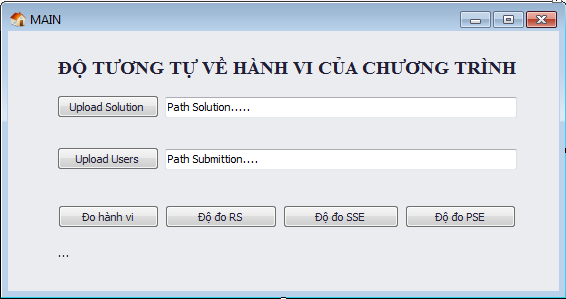
\includegraphics[width=0.8\linewidth]{images/main.png}
\begin{itemize}
	\item Hai nút Upload Solution và Upload Users cho phép tải 
	chương trình tham chiếu và chương trình cần tính
	\item Bên dưới là các nút đo độ tương tự hành vi của chương
	trình, và kết quả các phép đo RS, SSE và PSE.
\end{itemize}	
\end{block}
\end{frame}

\begin{frame}{Thực nghiệm, đánh giá}
\begin{block}{\ref{subsec:DGKQTN}. Kết quả thực nghiệm}
	\centering
	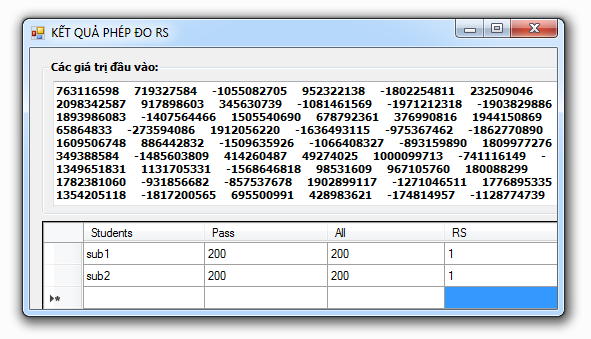
\includegraphics[width=0.6\linewidth]{images/kq_rs.png} \\	
	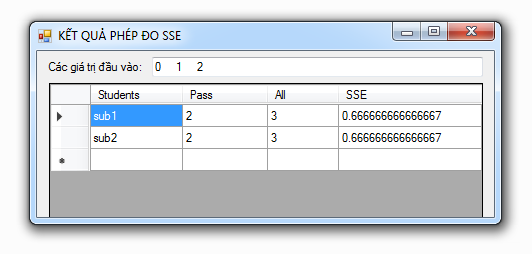
\includegraphics[width=0.6\linewidth]{images/kq_sse.png} \\
	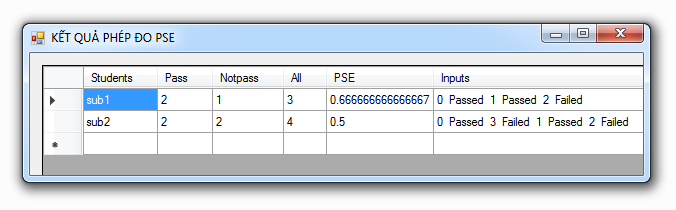
\includegraphics[width=0.6\linewidth]{images/kq_pse.png}	
\end{block}
\end{frame}

\begin{frame}{Thực nghiệm, đánh giá}
\begin{block}{\ref{subsec:DGKQTN}. Kết quả thực nghiệm}
\begin{itemize}
	\item Phép đo RS
	\begin{itemize}
		\item Ưu điểm: Đánh giá khách quan, tốc độ xử lý nhanh, 
		ít tốn tài nguyên máy tính
		\item Hạn chế: Không quan tâm đến hành vi của chương 
		trình, chỉ quan tâm đến dữ liệu vào và ra của chương trình
	\end{itemize} \pause
	\item Phép đo SSE
	\begin{itemize}
		\item Ưu điểm: Sử dụng kỹ thuật DSE để sinh ra tập các 
		giá trị đầu vào của chương trình, phép đo PSE cho kết quả 
		chính xác hơn phép đo RS
		\item Hạn chế: Không quan tâm đến chương trình cần phân tích, 
		tốn tài nguyên máy tính, thời gian thực thi chậm hơn phép đo RS
	\end{itemize} \pause
	\item Phép đo PSE
	\begin{itemize}
		\item Ưu điểm: Tập giá trị đầu vào của chương trình có độ phủ cao, 
		kết quả độ tương tự hành vi của chương trình theo phép đo PSE tốt hơn phép đo SSE
		\item Hạn chế: Tốn tài nguyên máy tính và thời 
		gian thực thi lâu hơn phép đo SSE
	\end{itemize}
\end{itemize}
\end{block}
\end{frame}

\subsection{Hướng phát triển và khả năng ứng dụng}
\label{subsec:HPTKNUD}
\subsubsection*{Hướng phát triển}
\label{subsubsec:HPT}
\subsubsection*{Khả năng ứng dụng}
\label{subsubsec:KNUD}
\begin{frame}{Hướng phát triển và khả năng ứng dụng}
	\begin{block}{\ref{subsubsec:HPT}. Hướng phát triển}
		\begin{itemize}
			\item Cải tiến các phép đo để kết quả được chính xác hơn
			\item Tích hợp thêm một số ngôn ngữ Java, C++...
		\end{itemize}
	\end{block} \pause
	\begin{block}{\ref{subsubsec:KNUD}. Khả năng ứng dụng}
		\begin{itemize}
			\item Đánh giá tiến bộ trong lập trình
			\item Xếp hạng tự động
			\item Gợi ý giải pháp lập trình
		\end{itemize}
	\end{block}
\end{frame}

\begin{frame}{KẾT THÚC}
\centering
{\Huge XIN CẢM ƠN!}
\end{frame}



\bibliographystyle{plain}
\bibliography{biblio}
%\nocite{*} % dùng tạm thời
%\appendix
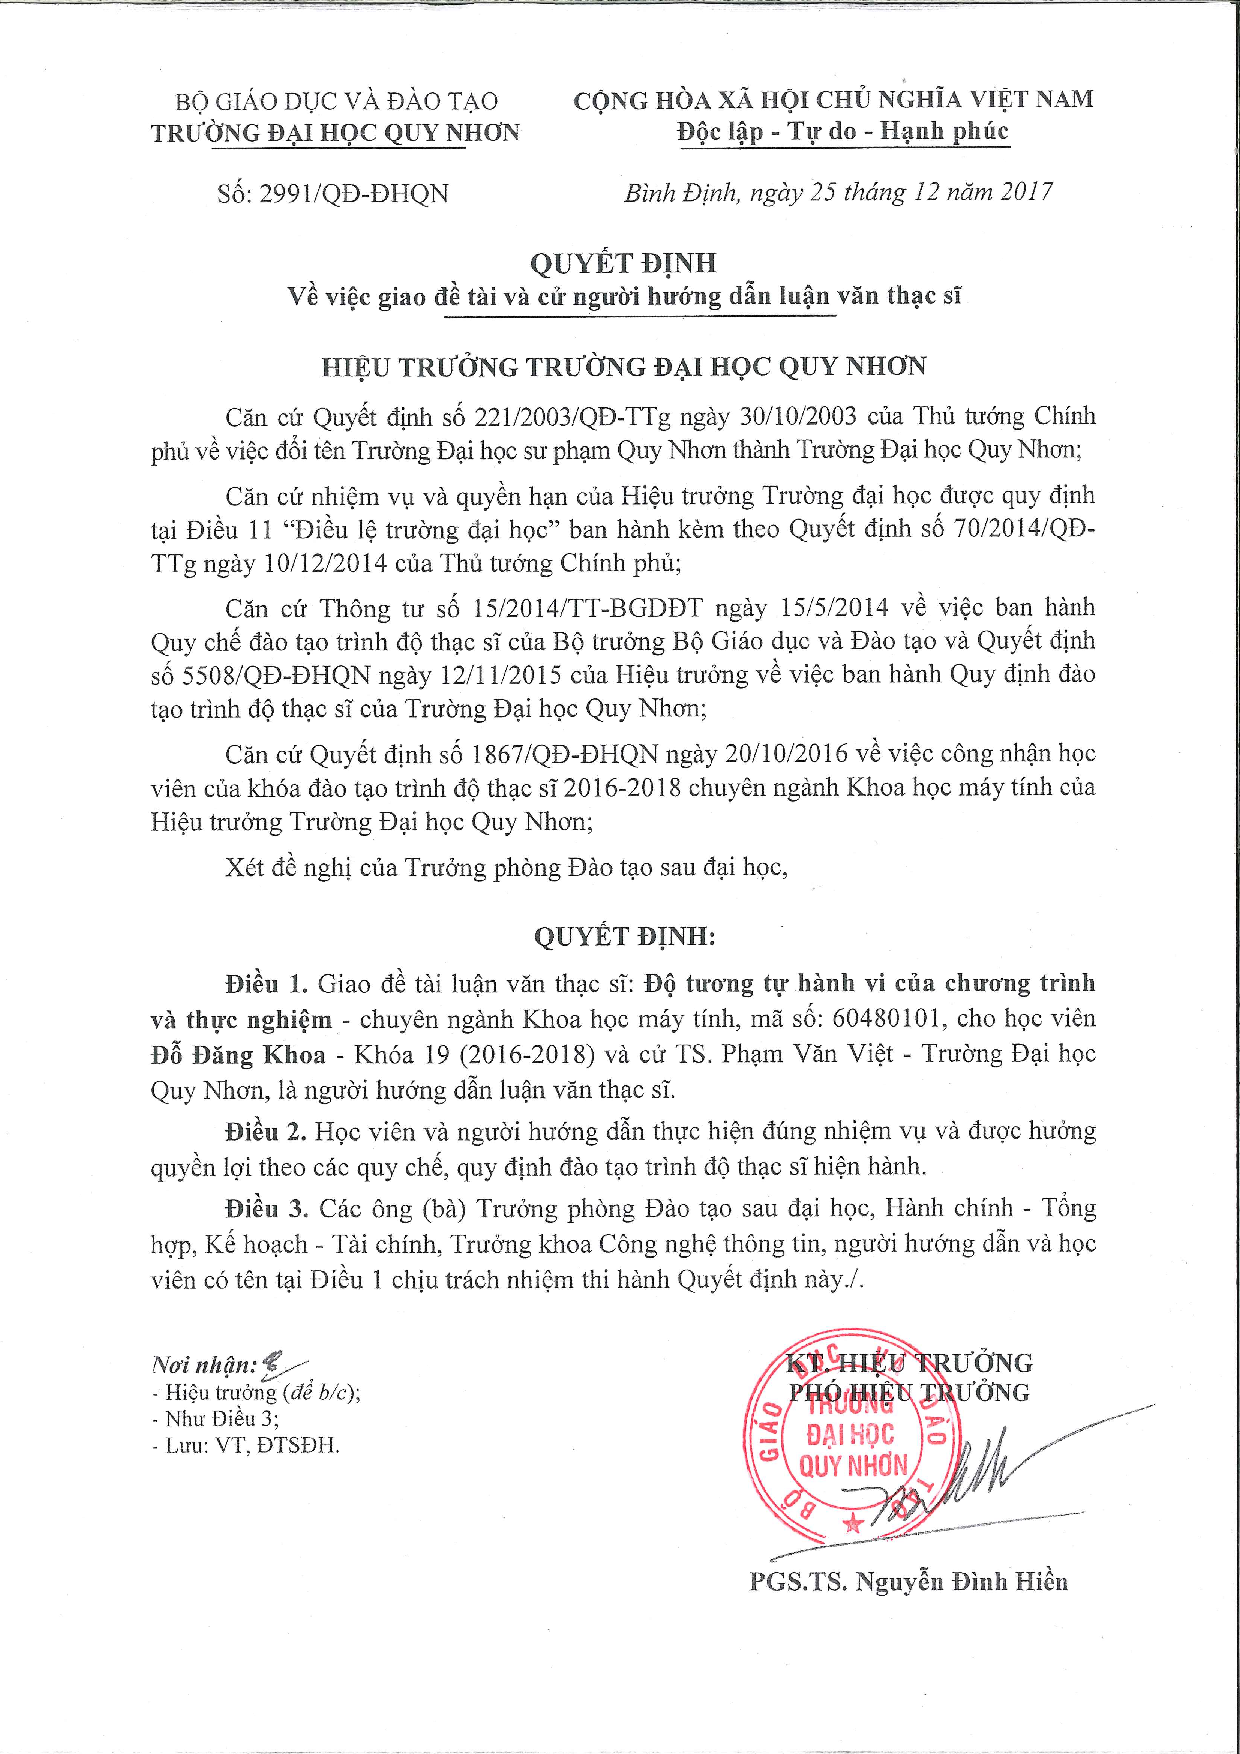
\includepdf{quyetdinh.pdf}
\chapter{MỘT SỐ MÃ LỆNH QUAN TRỌNG}
\lstinputlisting[caption = {Mã lệnh tạo project của sinh viên}]{MakeProjects.cs}

\lstinputlisting[caption= {Mã lệnh tạo project chương trình tham chiếu}]{MakeSecretProjects.cs}

\lstinputlisting[caption={Mã lệnh build project của sinh viên}]{BuildProjects.cs}

\lstinputlisting[caption={Mã lệnh build project chương trình tham chiếu}]{BuildSecretProjects.cs}

\lstinputlisting[caption={Mã lệnh build project chương trình hợp thành}]{BuildMetaProjects.cs}

\lstinputlisting[caption={Mã lệnh thực thi DSE trên chương trình hợp thành}]{RunPexOnMetaProjects.cs}

\lstinputlisting[caption={Mã lệnh phép đo RS}]{ComputeMetric3.cs}

\lstinputlisting[caption={Mã lệnh phép đo SSE}]{ComputeMetric2.cs}

\lstinputlisting[caption={Mã lệnh phép đo PSE}]{ComputeMetric1.cs}

 

\end{document}